\documentclass[11pt]{article}

    \usepackage[breakable]{tcolorbox}
    \usepackage{parskip} % Stop auto-indenting (to mimic markdown behaviour)
    
    \usepackage{iftex}
    \ifPDFTeX
    	\usepackage[T1]{fontenc}
    	\usepackage{mathpazo}
    \else
    	\usepackage{fontspec}
    \fi

    % Basic figure setup, for now with no caption control since it's done
    % automatically by Pandoc (which extracts ![](path) syntax from Markdown).
    \usepackage{graphicx}
    % Maintain compatibility with old templates. Remove in nbconvert 6.0
    \let\Oldincludegraphics\includegraphics
    % Ensure that by default, figures have no caption (until we provide a
    % proper Figure object with a Caption API and a way to capture that
    % in the conversion process - todo).
    \usepackage{caption}
    \DeclareCaptionFormat{nocaption}{}
    \captionsetup{format=nocaption,aboveskip=0pt,belowskip=0pt}

    \usepackage[Export]{adjustbox} % Used to constrain images to a maximum size
    \adjustboxset{max size={0.9\linewidth}{0.9\paperheight}}
    \usepackage{float}
    \floatplacement{figure}{H} % forces figures to be placed at the correct location
    \usepackage{xcolor} % Allow colors to be defined
    \usepackage{enumerate} % Needed for markdown enumerations to work
    \usepackage{geometry} % Used to adjust the document margins
    \usepackage{amsmath} % Equations
    \usepackage{amssymb} % Equations
    \usepackage{textcomp} % defines textquotesingle
    % Hack from http://tex.stackexchange.com/a/47451/13684:
    \AtBeginDocument{%
        \def\PYZsq{\textquotesingle}% Upright quotes in Pygmentized code
    }
    \usepackage{upquote} % Upright quotes for verbatim code
    \usepackage{eurosym} % defines \euro
    \usepackage[mathletters]{ucs} % Extended unicode (utf-8) support
    \usepackage{fancyvrb} % verbatim replacement that allows latex
    \usepackage{grffile} % extends the file name processing of package graphics 
                         % to support a larger range
    \makeatletter % fix for grffile with XeLaTeX
    \def\Gread@@xetex#1{%
      \IfFileExists{"\Gin@base".bb}%
      {\Gread@eps{\Gin@base.bb}}%
      {\Gread@@xetex@aux#1}%
    }
    \makeatother

    % The hyperref package gives us a pdf with properly built
    % internal navigation ('pdf bookmarks' for the table of contents,
    % internal cross-reference links, web links for URLs, etc.)
    \usepackage{hyperref}
    % The default LaTeX title has an obnoxious amount of whitespace. By default,
    % titling removes some of it. It also provides customization options.
    \usepackage{titling}
    \usepackage{longtable} % longtable support required by pandoc >1.10
    \usepackage{booktabs}  % table support for pandoc > 1.12.2
    \usepackage[inline]{enumitem} % IRkernel/repr support (it uses the enumerate* environment)
    \usepackage[normalem]{ulem} % ulem is needed to support strikethroughs (\sout)
                                % normalem makes italics be italics, not underlines
    \usepackage{mathrsfs}
    

    
    % Colors for the hyperref package
    \definecolor{urlcolor}{rgb}{0,.145,.698}
    \definecolor{linkcolor}{rgb}{.71,0.21,0.01}
    \definecolor{citecolor}{rgb}{.12,.54,.11}

    % ANSI colors
    \definecolor{ansi-black}{HTML}{3E424D}
    \definecolor{ansi-black-intense}{HTML}{282C36}
    \definecolor{ansi-red}{HTML}{E75C58}
    \definecolor{ansi-red-intense}{HTML}{B22B31}
    \definecolor{ansi-green}{HTML}{00A250}
    \definecolor{ansi-green-intense}{HTML}{007427}
    \definecolor{ansi-yellow}{HTML}{DDB62B}
    \definecolor{ansi-yellow-intense}{HTML}{B27D12}
    \definecolor{ansi-blue}{HTML}{208FFB}
    \definecolor{ansi-blue-intense}{HTML}{0065CA}
    \definecolor{ansi-magenta}{HTML}{D160C4}
    \definecolor{ansi-magenta-intense}{HTML}{A03196}
    \definecolor{ansi-cyan}{HTML}{60C6C8}
    \definecolor{ansi-cyan-intense}{HTML}{258F8F}
    \definecolor{ansi-white}{HTML}{C5C1B4}
    \definecolor{ansi-white-intense}{HTML}{A1A6B2}
    \definecolor{ansi-default-inverse-fg}{HTML}{FFFFFF}
    \definecolor{ansi-default-inverse-bg}{HTML}{000000}

    % commands and environments needed by pandoc snippets
    % extracted from the output of `pandoc -s`
    \providecommand{\tightlist}{%
      \setlength{\itemsep}{0pt}\setlength{\parskip}{0pt}}
    \DefineVerbatimEnvironment{Highlighting}{Verbatim}{commandchars=\\\{\}}
    % Add ',fontsize=\small' for more characters per line
    \newenvironment{Shaded}{}{}
    \newcommand{\KeywordTok}[1]{\textcolor[rgb]{0.00,0.44,0.13}{\textbf{{#1}}}}
    \newcommand{\DataTypeTok}[1]{\textcolor[rgb]{0.56,0.13,0.00}{{#1}}}
    \newcommand{\DecValTok}[1]{\textcolor[rgb]{0.25,0.63,0.44}{{#1}}}
    \newcommand{\BaseNTok}[1]{\textcolor[rgb]{0.25,0.63,0.44}{{#1}}}
    \newcommand{\FloatTok}[1]{\textcolor[rgb]{0.25,0.63,0.44}{{#1}}}
    \newcommand{\CharTok}[1]{\textcolor[rgb]{0.25,0.44,0.63}{{#1}}}
    \newcommand{\StringTok}[1]{\textcolor[rgb]{0.25,0.44,0.63}{{#1}}}
    \newcommand{\CommentTok}[1]{\textcolor[rgb]{0.38,0.63,0.69}{\textit{{#1}}}}
    \newcommand{\OtherTok}[1]{\textcolor[rgb]{0.00,0.44,0.13}{{#1}}}
    \newcommand{\AlertTok}[1]{\textcolor[rgb]{1.00,0.00,0.00}{\textbf{{#1}}}}
    \newcommand{\FunctionTok}[1]{\textcolor[rgb]{0.02,0.16,0.49}{{#1}}}
    \newcommand{\RegionMarkerTok}[1]{{#1}}
    \newcommand{\ErrorTok}[1]{\textcolor[rgb]{1.00,0.00,0.00}{\textbf{{#1}}}}
    \newcommand{\NormalTok}[1]{{#1}}
    
    % Additional commands for more recent versions of Pandoc
    \newcommand{\ConstantTok}[1]{\textcolor[rgb]{0.53,0.00,0.00}{{#1}}}
    \newcommand{\SpecialCharTok}[1]{\textcolor[rgb]{0.25,0.44,0.63}{{#1}}}
    \newcommand{\VerbatimStringTok}[1]{\textcolor[rgb]{0.25,0.44,0.63}{{#1}}}
    \newcommand{\SpecialStringTok}[1]{\textcolor[rgb]{0.73,0.40,0.53}{{#1}}}
    \newcommand{\ImportTok}[1]{{#1}}
    \newcommand{\DocumentationTok}[1]{\textcolor[rgb]{0.73,0.13,0.13}{\textit{{#1}}}}
    \newcommand{\AnnotationTok}[1]{\textcolor[rgb]{0.38,0.63,0.69}{\textbf{\textit{{#1}}}}}
    \newcommand{\CommentVarTok}[1]{\textcolor[rgb]{0.38,0.63,0.69}{\textbf{\textit{{#1}}}}}
    \newcommand{\VariableTok}[1]{\textcolor[rgb]{0.10,0.09,0.49}{{#1}}}
    \newcommand{\ControlFlowTok}[1]{\textcolor[rgb]{0.00,0.44,0.13}{\textbf{{#1}}}}
    \newcommand{\OperatorTok}[1]{\textcolor[rgb]{0.40,0.40,0.40}{{#1}}}
    \newcommand{\BuiltInTok}[1]{{#1}}
    \newcommand{\ExtensionTok}[1]{{#1}}
    \newcommand{\PreprocessorTok}[1]{\textcolor[rgb]{0.74,0.48,0.00}{{#1}}}
    \newcommand{\AttributeTok}[1]{\textcolor[rgb]{0.49,0.56,0.16}{{#1}}}
    \newcommand{\InformationTok}[1]{\textcolor[rgb]{0.38,0.63,0.69}{\textbf{\textit{{#1}}}}}
    \newcommand{\WarningTok}[1]{\textcolor[rgb]{0.38,0.63,0.69}{\textbf{\textit{{#1}}}}}
    
    
    % Define a nice break command that doesn't care if a line doesn't already
    % exist.
    \def\br{\hspace*{\fill} \\* }
    % Math Jax compatibility definitions
    \def\gt{>}
    \def\lt{<}
    \let\Oldtex\TeX
    \let\Oldlatex\LaTeX
    \renewcommand{\TeX}{\textrm{\Oldtex}}
    \renewcommand{\LaTeX}{\textrm{\Oldlatex}}
    % Document parameters
    % Document title
    \title{trigger\_word\_detection}
    
    
    
    
    
% Pygments definitions
\makeatletter
\def\PY@reset{\let\PY@it=\relax \let\PY@bf=\relax%
    \let\PY@ul=\relax \let\PY@tc=\relax%
    \let\PY@bc=\relax \let\PY@ff=\relax}
\def\PY@tok#1{\csname PY@tok@#1\endcsname}
\def\PY@toks#1+{\ifx\relax#1\empty\else%
    \PY@tok{#1}\expandafter\PY@toks\fi}
\def\PY@do#1{\PY@bc{\PY@tc{\PY@ul{%
    \PY@it{\PY@bf{\PY@ff{#1}}}}}}}
\def\PY#1#2{\PY@reset\PY@toks#1+\relax+\PY@do{#2}}

\expandafter\def\csname PY@tok@w\endcsname{\def\PY@tc##1{\textcolor[rgb]{0.73,0.73,0.73}{##1}}}
\expandafter\def\csname PY@tok@c\endcsname{\let\PY@it=\textit\def\PY@tc##1{\textcolor[rgb]{0.25,0.50,0.50}{##1}}}
\expandafter\def\csname PY@tok@cp\endcsname{\def\PY@tc##1{\textcolor[rgb]{0.74,0.48,0.00}{##1}}}
\expandafter\def\csname PY@tok@k\endcsname{\let\PY@bf=\textbf\def\PY@tc##1{\textcolor[rgb]{0.00,0.50,0.00}{##1}}}
\expandafter\def\csname PY@tok@kp\endcsname{\def\PY@tc##1{\textcolor[rgb]{0.00,0.50,0.00}{##1}}}
\expandafter\def\csname PY@tok@kt\endcsname{\def\PY@tc##1{\textcolor[rgb]{0.69,0.00,0.25}{##1}}}
\expandafter\def\csname PY@tok@o\endcsname{\def\PY@tc##1{\textcolor[rgb]{0.40,0.40,0.40}{##1}}}
\expandafter\def\csname PY@tok@ow\endcsname{\let\PY@bf=\textbf\def\PY@tc##1{\textcolor[rgb]{0.67,0.13,1.00}{##1}}}
\expandafter\def\csname PY@tok@nb\endcsname{\def\PY@tc##1{\textcolor[rgb]{0.00,0.50,0.00}{##1}}}
\expandafter\def\csname PY@tok@nf\endcsname{\def\PY@tc##1{\textcolor[rgb]{0.00,0.00,1.00}{##1}}}
\expandafter\def\csname PY@tok@nc\endcsname{\let\PY@bf=\textbf\def\PY@tc##1{\textcolor[rgb]{0.00,0.00,1.00}{##1}}}
\expandafter\def\csname PY@tok@nn\endcsname{\let\PY@bf=\textbf\def\PY@tc##1{\textcolor[rgb]{0.00,0.00,1.00}{##1}}}
\expandafter\def\csname PY@tok@ne\endcsname{\let\PY@bf=\textbf\def\PY@tc##1{\textcolor[rgb]{0.82,0.25,0.23}{##1}}}
\expandafter\def\csname PY@tok@nv\endcsname{\def\PY@tc##1{\textcolor[rgb]{0.10,0.09,0.49}{##1}}}
\expandafter\def\csname PY@tok@no\endcsname{\def\PY@tc##1{\textcolor[rgb]{0.53,0.00,0.00}{##1}}}
\expandafter\def\csname PY@tok@nl\endcsname{\def\PY@tc##1{\textcolor[rgb]{0.63,0.63,0.00}{##1}}}
\expandafter\def\csname PY@tok@ni\endcsname{\let\PY@bf=\textbf\def\PY@tc##1{\textcolor[rgb]{0.60,0.60,0.60}{##1}}}
\expandafter\def\csname PY@tok@na\endcsname{\def\PY@tc##1{\textcolor[rgb]{0.49,0.56,0.16}{##1}}}
\expandafter\def\csname PY@tok@nt\endcsname{\let\PY@bf=\textbf\def\PY@tc##1{\textcolor[rgb]{0.00,0.50,0.00}{##1}}}
\expandafter\def\csname PY@tok@nd\endcsname{\def\PY@tc##1{\textcolor[rgb]{0.67,0.13,1.00}{##1}}}
\expandafter\def\csname PY@tok@s\endcsname{\def\PY@tc##1{\textcolor[rgb]{0.73,0.13,0.13}{##1}}}
\expandafter\def\csname PY@tok@sd\endcsname{\let\PY@it=\textit\def\PY@tc##1{\textcolor[rgb]{0.73,0.13,0.13}{##1}}}
\expandafter\def\csname PY@tok@si\endcsname{\let\PY@bf=\textbf\def\PY@tc##1{\textcolor[rgb]{0.73,0.40,0.53}{##1}}}
\expandafter\def\csname PY@tok@se\endcsname{\let\PY@bf=\textbf\def\PY@tc##1{\textcolor[rgb]{0.73,0.40,0.13}{##1}}}
\expandafter\def\csname PY@tok@sr\endcsname{\def\PY@tc##1{\textcolor[rgb]{0.73,0.40,0.53}{##1}}}
\expandafter\def\csname PY@tok@ss\endcsname{\def\PY@tc##1{\textcolor[rgb]{0.10,0.09,0.49}{##1}}}
\expandafter\def\csname PY@tok@sx\endcsname{\def\PY@tc##1{\textcolor[rgb]{0.00,0.50,0.00}{##1}}}
\expandafter\def\csname PY@tok@m\endcsname{\def\PY@tc##1{\textcolor[rgb]{0.40,0.40,0.40}{##1}}}
\expandafter\def\csname PY@tok@gh\endcsname{\let\PY@bf=\textbf\def\PY@tc##1{\textcolor[rgb]{0.00,0.00,0.50}{##1}}}
\expandafter\def\csname PY@tok@gu\endcsname{\let\PY@bf=\textbf\def\PY@tc##1{\textcolor[rgb]{0.50,0.00,0.50}{##1}}}
\expandafter\def\csname PY@tok@gd\endcsname{\def\PY@tc##1{\textcolor[rgb]{0.63,0.00,0.00}{##1}}}
\expandafter\def\csname PY@tok@gi\endcsname{\def\PY@tc##1{\textcolor[rgb]{0.00,0.63,0.00}{##1}}}
\expandafter\def\csname PY@tok@gr\endcsname{\def\PY@tc##1{\textcolor[rgb]{1.00,0.00,0.00}{##1}}}
\expandafter\def\csname PY@tok@ge\endcsname{\let\PY@it=\textit}
\expandafter\def\csname PY@tok@gs\endcsname{\let\PY@bf=\textbf}
\expandafter\def\csname PY@tok@gp\endcsname{\let\PY@bf=\textbf\def\PY@tc##1{\textcolor[rgb]{0.00,0.00,0.50}{##1}}}
\expandafter\def\csname PY@tok@go\endcsname{\def\PY@tc##1{\textcolor[rgb]{0.53,0.53,0.53}{##1}}}
\expandafter\def\csname PY@tok@gt\endcsname{\def\PY@tc##1{\textcolor[rgb]{0.00,0.27,0.87}{##1}}}
\expandafter\def\csname PY@tok@err\endcsname{\def\PY@bc##1{\setlength{\fboxsep}{0pt}\fcolorbox[rgb]{1.00,0.00,0.00}{1,1,1}{\strut ##1}}}
\expandafter\def\csname PY@tok@kc\endcsname{\let\PY@bf=\textbf\def\PY@tc##1{\textcolor[rgb]{0.00,0.50,0.00}{##1}}}
\expandafter\def\csname PY@tok@kd\endcsname{\let\PY@bf=\textbf\def\PY@tc##1{\textcolor[rgb]{0.00,0.50,0.00}{##1}}}
\expandafter\def\csname PY@tok@kn\endcsname{\let\PY@bf=\textbf\def\PY@tc##1{\textcolor[rgb]{0.00,0.50,0.00}{##1}}}
\expandafter\def\csname PY@tok@kr\endcsname{\let\PY@bf=\textbf\def\PY@tc##1{\textcolor[rgb]{0.00,0.50,0.00}{##1}}}
\expandafter\def\csname PY@tok@bp\endcsname{\def\PY@tc##1{\textcolor[rgb]{0.00,0.50,0.00}{##1}}}
\expandafter\def\csname PY@tok@fm\endcsname{\def\PY@tc##1{\textcolor[rgb]{0.00,0.00,1.00}{##1}}}
\expandafter\def\csname PY@tok@vc\endcsname{\def\PY@tc##1{\textcolor[rgb]{0.10,0.09,0.49}{##1}}}
\expandafter\def\csname PY@tok@vg\endcsname{\def\PY@tc##1{\textcolor[rgb]{0.10,0.09,0.49}{##1}}}
\expandafter\def\csname PY@tok@vi\endcsname{\def\PY@tc##1{\textcolor[rgb]{0.10,0.09,0.49}{##1}}}
\expandafter\def\csname PY@tok@vm\endcsname{\def\PY@tc##1{\textcolor[rgb]{0.10,0.09,0.49}{##1}}}
\expandafter\def\csname PY@tok@sa\endcsname{\def\PY@tc##1{\textcolor[rgb]{0.73,0.13,0.13}{##1}}}
\expandafter\def\csname PY@tok@sb\endcsname{\def\PY@tc##1{\textcolor[rgb]{0.73,0.13,0.13}{##1}}}
\expandafter\def\csname PY@tok@sc\endcsname{\def\PY@tc##1{\textcolor[rgb]{0.73,0.13,0.13}{##1}}}
\expandafter\def\csname PY@tok@dl\endcsname{\def\PY@tc##1{\textcolor[rgb]{0.73,0.13,0.13}{##1}}}
\expandafter\def\csname PY@tok@s2\endcsname{\def\PY@tc##1{\textcolor[rgb]{0.73,0.13,0.13}{##1}}}
\expandafter\def\csname PY@tok@sh\endcsname{\def\PY@tc##1{\textcolor[rgb]{0.73,0.13,0.13}{##1}}}
\expandafter\def\csname PY@tok@s1\endcsname{\def\PY@tc##1{\textcolor[rgb]{0.73,0.13,0.13}{##1}}}
\expandafter\def\csname PY@tok@mb\endcsname{\def\PY@tc##1{\textcolor[rgb]{0.40,0.40,0.40}{##1}}}
\expandafter\def\csname PY@tok@mf\endcsname{\def\PY@tc##1{\textcolor[rgb]{0.40,0.40,0.40}{##1}}}
\expandafter\def\csname PY@tok@mh\endcsname{\def\PY@tc##1{\textcolor[rgb]{0.40,0.40,0.40}{##1}}}
\expandafter\def\csname PY@tok@mi\endcsname{\def\PY@tc##1{\textcolor[rgb]{0.40,0.40,0.40}{##1}}}
\expandafter\def\csname PY@tok@il\endcsname{\def\PY@tc##1{\textcolor[rgb]{0.40,0.40,0.40}{##1}}}
\expandafter\def\csname PY@tok@mo\endcsname{\def\PY@tc##1{\textcolor[rgb]{0.40,0.40,0.40}{##1}}}
\expandafter\def\csname PY@tok@ch\endcsname{\let\PY@it=\textit\def\PY@tc##1{\textcolor[rgb]{0.25,0.50,0.50}{##1}}}
\expandafter\def\csname PY@tok@cm\endcsname{\let\PY@it=\textit\def\PY@tc##1{\textcolor[rgb]{0.25,0.50,0.50}{##1}}}
\expandafter\def\csname PY@tok@cpf\endcsname{\let\PY@it=\textit\def\PY@tc##1{\textcolor[rgb]{0.25,0.50,0.50}{##1}}}
\expandafter\def\csname PY@tok@c1\endcsname{\let\PY@it=\textit\def\PY@tc##1{\textcolor[rgb]{0.25,0.50,0.50}{##1}}}
\expandafter\def\csname PY@tok@cs\endcsname{\let\PY@it=\textit\def\PY@tc##1{\textcolor[rgb]{0.25,0.50,0.50}{##1}}}

\def\PYZbs{\char`\\}
\def\PYZus{\char`\_}
\def\PYZob{\char`\{}
\def\PYZcb{\char`\}}
\def\PYZca{\char`\^}
\def\PYZam{\char`\&}
\def\PYZlt{\char`\<}
\def\PYZgt{\char`\>}
\def\PYZsh{\char`\#}
\def\PYZpc{\char`\%}
\def\PYZdl{\char`\$}
\def\PYZhy{\char`\-}
\def\PYZsq{\char`\'}
\def\PYZdq{\char`\"}
\def\PYZti{\char`\~}
% for compatibility with earlier versions
\def\PYZat{@}
\def\PYZlb{[}
\def\PYZrb{]}
\makeatother


    % For linebreaks inside Verbatim environment from package fancyvrb. 
    \makeatletter
        \newbox\Wrappedcontinuationbox 
        \newbox\Wrappedvisiblespacebox 
        \newcommand*\Wrappedvisiblespace {\textcolor{red}{\textvisiblespace}} 
        \newcommand*\Wrappedcontinuationsymbol {\textcolor{red}{\llap{\tiny$\m@th\hookrightarrow$}}} 
        \newcommand*\Wrappedcontinuationindent {3ex } 
        \newcommand*\Wrappedafterbreak {\kern\Wrappedcontinuationindent\copy\Wrappedcontinuationbox} 
        % Take advantage of the already applied Pygments mark-up to insert 
        % potential linebreaks for TeX processing. 
        %        {, <, #, %, $, ' and ": go to next line. 
        %        _, }, ^, &, >, - and ~: stay at end of broken line. 
        % Use of \textquotesingle for straight quote. 
        \newcommand*\Wrappedbreaksatspecials {% 
            \def\PYGZus{\discretionary{\char`\_}{\Wrappedafterbreak}{\char`\_}}% 
            \def\PYGZob{\discretionary{}{\Wrappedafterbreak\char`\{}{\char`\{}}% 
            \def\PYGZcb{\discretionary{\char`\}}{\Wrappedafterbreak}{\char`\}}}% 
            \def\PYGZca{\discretionary{\char`\^}{\Wrappedafterbreak}{\char`\^}}% 
            \def\PYGZam{\discretionary{\char`\&}{\Wrappedafterbreak}{\char`\&}}% 
            \def\PYGZlt{\discretionary{}{\Wrappedafterbreak\char`\<}{\char`\<}}% 
            \def\PYGZgt{\discretionary{\char`\>}{\Wrappedafterbreak}{\char`\>}}% 
            \def\PYGZsh{\discretionary{}{\Wrappedafterbreak\char`\#}{\char`\#}}% 
            \def\PYGZpc{\discretionary{}{\Wrappedafterbreak\char`\%}{\char`\%}}% 
            \def\PYGZdl{\discretionary{}{\Wrappedafterbreak\char`\$}{\char`\$}}% 
            \def\PYGZhy{\discretionary{\char`\-}{\Wrappedafterbreak}{\char`\-}}% 
            \def\PYGZsq{\discretionary{}{\Wrappedafterbreak\textquotesingle}{\textquotesingle}}% 
            \def\PYGZdq{\discretionary{}{\Wrappedafterbreak\char`\"}{\char`\"}}% 
            \def\PYGZti{\discretionary{\char`\~}{\Wrappedafterbreak}{\char`\~}}% 
        } 
        % Some characters . , ; ? ! / are not pygmentized. 
        % This macro makes them "active" and they will insert potential linebreaks 
        \newcommand*\Wrappedbreaksatpunct {% 
            \lccode`\~`\.\lowercase{\def~}{\discretionary{\hbox{\char`\.}}{\Wrappedafterbreak}{\hbox{\char`\.}}}% 
            \lccode`\~`\,\lowercase{\def~}{\discretionary{\hbox{\char`\,}}{\Wrappedafterbreak}{\hbox{\char`\,}}}% 
            \lccode`\~`\;\lowercase{\def~}{\discretionary{\hbox{\char`\;}}{\Wrappedafterbreak}{\hbox{\char`\;}}}% 
            \lccode`\~`\:\lowercase{\def~}{\discretionary{\hbox{\char`\:}}{\Wrappedafterbreak}{\hbox{\char`\:}}}% 
            \lccode`\~`\?\lowercase{\def~}{\discretionary{\hbox{\char`\?}}{\Wrappedafterbreak}{\hbox{\char`\?}}}% 
            \lccode`\~`\!\lowercase{\def~}{\discretionary{\hbox{\char`\!}}{\Wrappedafterbreak}{\hbox{\char`\!}}}% 
            \lccode`\~`\/\lowercase{\def~}{\discretionary{\hbox{\char`\/}}{\Wrappedafterbreak}{\hbox{\char`\/}}}% 
            \catcode`\.\active
            \catcode`\,\active 
            \catcode`\;\active
            \catcode`\:\active
            \catcode`\?\active
            \catcode`\!\active
            \catcode`\/\active 
            \lccode`\~`\~ 	
        }
    \makeatother

    \let\OriginalVerbatim=\Verbatim
    \makeatletter
    \renewcommand{\Verbatim}[1][1]{%
        %\parskip\z@skip
        \sbox\Wrappedcontinuationbox {\Wrappedcontinuationsymbol}%
        \sbox\Wrappedvisiblespacebox {\FV@SetupFont\Wrappedvisiblespace}%
        \def\FancyVerbFormatLine ##1{\hsize\linewidth
            \vtop{\raggedright\hyphenpenalty\z@\exhyphenpenalty\z@
                \doublehyphendemerits\z@\finalhyphendemerits\z@
                \strut ##1\strut}%
        }%
        % If the linebreak is at a space, the latter will be displayed as visible
        % space at end of first line, and a continuation symbol starts next line.
        % Stretch/shrink are however usually zero for typewriter font.
        \def\FV@Space {%
            \nobreak\hskip\z@ plus\fontdimen3\font minus\fontdimen4\font
            \discretionary{\copy\Wrappedvisiblespacebox}{\Wrappedafterbreak}
            {\kern\fontdimen2\font}%
        }%
        
        % Allow breaks at special characters using \PYG... macros.
        \Wrappedbreaksatspecials
        % Breaks at punctuation characters . , ; ? ! and / need catcode=\active 	
        \OriginalVerbatim[#1,codes*=\Wrappedbreaksatpunct]%
    }
    \makeatother

    % Exact colors from NB
    \definecolor{incolor}{HTML}{303F9F}
    \definecolor{outcolor}{HTML}{D84315}
    \definecolor{cellborder}{HTML}{CFCFCF}
    \definecolor{cellbackground}{HTML}{F7F7F7}
    
    % prompt
    \makeatletter
    \newcommand{\boxspacing}{\kern\kvtcb@left@rule\kern\kvtcb@boxsep}
    \makeatother
    \newcommand{\prompt}[4]{
        \ttfamily\llap{{\color{#2}[#3]:\hspace{3pt}#4}}\vspace{-\baselineskip}
    }
    

    
    % Prevent overflowing lines due to hard-to-break entities
    \sloppy 
    % Setup hyperref package
    \hypersetup{
      breaklinks=true,  % so long urls are correctly broken across lines
      colorlinks=true,
      urlcolor=urlcolor,
      linkcolor=linkcolor,
      citecolor=citecolor,
      }
    % Slightly bigger margins than the latex defaults
    
    \geometry{verbose,tmargin=1in,bmargin=1in,lmargin=1in,rmargin=1in}
    
    

\begin{document}
    
    \maketitle
    
    

    
    Project created during the Deep Learning Specialization course on
www.coursera.or

    \hypertarget{trigger-word-detection}{%
\section{Trigger word detection}\label{trigger-word-detection}}

    \begin{tcolorbox}[breakable, size=fbox, boxrule=1pt, pad at break*=1mm,colback=cellbackground, colframe=cellborder]
\prompt{In}{incolor}{1}{\boxspacing}
\begin{Verbatim}[commandchars=\\\{\}]
\PY{k+kn}{import} \PY{n+nn}{numpy} \PY{k}{as} \PY{n+nn}{np}
\PY{k+kn}{from} \PY{n+nn}{pydub} \PY{k+kn}{import} \PY{n}{AudioSegment} \PY{c+c1}{\PYZsh{} Audio files editing}
\PY{k+kn}{import} \PY{n+nn}{random}
\PY{k+kn}{import} \PY{n+nn}{sys}
\PY{k+kn}{import} \PY{n+nn}{io}
\PY{k+kn}{import} \PY{n+nn}{os}
\PY{k+kn}{from} \PY{n+nn}{scipy}\PY{n+nn}{.}\PY{n+nn}{io} \PY{k+kn}{import} \PY{n}{wavfile}
\PY{k+kn}{import} \PY{n+nn}{glob} \PY{c+c1}{\PYZsh{} Finds pathnames matching a pattern}
\PY{k+kn}{import} \PY{n+nn}{IPython} \PY{c+c1}{\PYZsh{} Interactive Python}
\PY{k+kn}{import} \PY{n+nn}{matplotlib}\PY{n+nn}{.}\PY{n+nn}{pyplot} \PY{k}{as} \PY{n+nn}{plt}
\PY{o}{\PYZpc{}}\PY{k}{matplotlib} inline 
\end{Verbatim}
\end{tcolorbox}

    \hypertarget{data-preparation}{%
\subsection{Data preparation}\label{data-preparation}}

    \begin{tcolorbox}[breakable, size=fbox, boxrule=1pt, pad at break*=1mm,colback=cellbackground, colframe=cellborder]
\prompt{In}{incolor}{2}{\boxspacing}
\begin{Verbatim}[commandchars=\\\{\}]
\PY{c+c1}{\PYZsh{} Exampleo of a trigger word}
\PY{n}{IPython}\PY{o}{.}\PY{n}{display}\PY{o}{.}\PY{n}{Audio}\PY{p}{(}\PY{l+s+s1}{\PYZsq{}}\PY{l+s+s1}{./raw\PYZus{}data/activates/1.wav}\PY{l+s+s1}{\PYZsq{}}\PY{p}{)}
\end{Verbatim}
\end{tcolorbox}

            \begin{tcolorbox}[breakable, size=fbox, boxrule=.5pt, pad at break*=1mm, opacityfill=0]
\prompt{Out}{outcolor}{2}{\boxspacing}
\begin{Verbatim}[commandchars=\\\{\}]
<IPython.lib.display.Audio object>
\end{Verbatim}
\end{tcolorbox}
        
    \begin{tcolorbox}[breakable, size=fbox, boxrule=1pt, pad at break*=1mm,colback=cellbackground, colframe=cellborder]
\prompt{In}{incolor}{3}{\boxspacing}
\begin{Verbatim}[commandchars=\\\{\}]
\PY{c+c1}{\PYZsh{} Example of a non\PYZhy{}trigger word}
\PY{n}{IPython}\PY{o}{.}\PY{n}{display}\PY{o}{.}\PY{n}{Audio}\PY{p}{(}\PY{l+s+s1}{\PYZsq{}}\PY{l+s+s1}{./raw\PYZus{}data/negatives/4.wav}\PY{l+s+s1}{\PYZsq{}}\PY{p}{)}
\end{Verbatim}
\end{tcolorbox}

            \begin{tcolorbox}[breakable, size=fbox, boxrule=.5pt, pad at break*=1mm, opacityfill=0]
\prompt{Out}{outcolor}{3}{\boxspacing}
\begin{Verbatim}[commandchars=\\\{\}]
<IPython.lib.display.Audio object>
\end{Verbatim}
\end{tcolorbox}
        
    \begin{tcolorbox}[breakable, size=fbox, boxrule=1pt, pad at break*=1mm,colback=cellbackground, colframe=cellborder]
\prompt{In}{incolor}{4}{\boxspacing}
\begin{Verbatim}[commandchars=\\\{\}]
\PY{c+c1}{\PYZsh{} Example of a background noise }
\PY{n}{IPython}\PY{o}{.}\PY{n}{display}\PY{o}{.}\PY{n}{Audio}\PY{p}{(}\PY{l+s+s1}{\PYZsq{}}\PY{l+s+s1}{./raw\PYZus{}data/backgrounds/1.wav}\PY{l+s+s1}{\PYZsq{}}\PY{p}{)}
\end{Verbatim}
\end{tcolorbox}

            \begin{tcolorbox}[breakable, size=fbox, boxrule=.5pt, pad at break*=1mm, opacityfill=0]
\prompt{Out}{outcolor}{4}{\boxspacing}
\begin{Verbatim}[commandchars=\\\{\}]
<IPython.lib.display.Audio object>
\end{Verbatim}
\end{tcolorbox}
        
    \begin{tcolorbox}[breakable, size=fbox, boxrule=1pt, pad at break*=1mm,colback=cellbackground, colframe=cellborder]
\prompt{In}{incolor}{5}{\boxspacing}
\begin{Verbatim}[commandchars=\\\{\}]
\PY{c+c1}{\PYZsh{} Load raw audio clips }

\PY{k}{def} \PY{n+nf}{load\PYZus{}raw\PYZus{}audio}\PY{p}{(}\PY{p}{)}\PY{p}{:}
    
    \PY{c+c1}{\PYZsh{} Initialize lists to store clips}
    \PY{n}{activates} \PY{o}{=} \PY{p}{[}\PY{p}{]}
    \PY{n}{backgrounds} \PY{o}{=} \PY{p}{[}\PY{p}{]}
    \PY{n}{negatives} \PY{o}{=} \PY{p}{[}\PY{p}{]}
    
    \PY{c+c1}{\PYZsh{} Load audio files in a list}
    
    \PY{c+c1}{\PYZsh{} Number of timesteps varies depending on a file}
    \PY{k}{for} \PY{n}{filename} \PY{o+ow}{in} \PY{n}{os}\PY{o}{.}\PY{n}{listdir}\PY{p}{(}\PY{l+s+s2}{\PYZdq{}}\PY{l+s+s2}{./raw\PYZus{}data/activates}\PY{l+s+s2}{\PYZdq{}}\PY{p}{)}\PY{p}{:}
        \PY{k}{if} \PY{n}{filename}\PY{o}{.}\PY{n}{endswith}\PY{p}{(}\PY{l+s+s2}{\PYZdq{}}\PY{l+s+s2}{wav}\PY{l+s+s2}{\PYZdq{}}\PY{p}{)}\PY{p}{:}
            \PY{n}{activate} \PY{o}{=} \PY{n}{AudioSegment}\PY{o}{.}\PY{n}{from\PYZus{}wav}\PY{p}{(}\PY{l+s+s2}{\PYZdq{}}\PY{l+s+s2}{./raw\PYZus{}data/activates/}\PY{l+s+s2}{\PYZdq{}}\PY{o}{+}\PY{n}{filename}\PY{p}{)}
            \PY{n}{activates}\PY{o}{.}\PY{n}{append}\PY{p}{(}\PY{n}{activate}\PY{p}{)}
    \PY{k}{for} \PY{n}{filename} \PY{o+ow}{in} \PY{n}{os}\PY{o}{.}\PY{n}{listdir}\PY{p}{(}\PY{l+s+s2}{\PYZdq{}}\PY{l+s+s2}{./raw\PYZus{}data/backgrounds}\PY{l+s+s2}{\PYZdq{}}\PY{p}{)}\PY{p}{:}
        
        \PY{c+c1}{\PYZsh{} (10 s clip / 0.001 s) (1 ms discretization of pydub) =\PYZgt{} 10000 timesteps}
        \PY{k}{if} \PY{n}{filename}\PY{o}{.}\PY{n}{endswith}\PY{p}{(}\PY{l+s+s2}{\PYZdq{}}\PY{l+s+s2}{wav}\PY{l+s+s2}{\PYZdq{}}\PY{p}{)}\PY{p}{:}
            \PY{n}{background} \PY{o}{=} \PY{n}{AudioSegment}\PY{o}{.}\PY{n}{from\PYZus{}wav}\PY{p}{(}\PY{l+s+s2}{\PYZdq{}}\PY{l+s+s2}{./raw\PYZus{}data/backgrounds/}\PY{l+s+s2}{\PYZdq{}}\PY{o}{+}\PY{n}{filename}\PY{p}{)}
            \PY{n}{backgrounds}\PY{o}{.}\PY{n}{append}\PY{p}{(}\PY{n}{background}\PY{p}{)}
            
    \PY{c+c1}{\PYZsh{} Number of timesteps varies depending on a file}
    \PY{k}{for} \PY{n}{filename} \PY{o+ow}{in} \PY{n}{os}\PY{o}{.}\PY{n}{listdir}\PY{p}{(}\PY{l+s+s2}{\PYZdq{}}\PY{l+s+s2}{./raw\PYZus{}data/negatives}\PY{l+s+s2}{\PYZdq{}}\PY{p}{)}\PY{p}{:}
        \PY{k}{if} \PY{n}{filename}\PY{o}{.}\PY{n}{endswith}\PY{p}{(}\PY{l+s+s2}{\PYZdq{}}\PY{l+s+s2}{wav}\PY{l+s+s2}{\PYZdq{}}\PY{p}{)}\PY{p}{:}
            \PY{n}{negative} \PY{o}{=} \PY{n}{AudioSegment}\PY{o}{.}\PY{n}{from\PYZus{}wav}\PY{p}{(}\PY{l+s+s2}{\PYZdq{}}\PY{l+s+s2}{./raw\PYZus{}data/negatives/}\PY{l+s+s2}{\PYZdq{}}\PY{o}{+}\PY{n}{filename}\PY{p}{)}
            \PY{n}{negatives}\PY{o}{.}\PY{n}{append}\PY{p}{(}\PY{n}{negative}\PY{p}{)}
            
    \PY{k}{return} \PY{n}{activates}\PY{p}{,} \PY{n}{negatives}\PY{p}{,} \PY{n}{backgrounds}
\end{Verbatim}
\end{tcolorbox}

    \begin{tcolorbox}[breakable, size=fbox, boxrule=1pt, pad at break*=1mm,colback=cellbackground, colframe=cellborder]
\prompt{In}{incolor}{6}{\boxspacing}
\begin{Verbatim}[commandchars=\\\{\}]
\PY{c+c1}{\PYZsh{} Load audio segments using pydub }
\PY{n}{activates}\PY{p}{,} \PY{n}{negatives}\PY{p}{,} \PY{n}{backgrounds} \PY{o}{=} \PY{n}{load\PYZus{}raw\PYZus{}audio}\PY{p}{(}\PY{p}{)}
\end{Verbatim}
\end{tcolorbox}

    \hypertarget{data-synthesis}{%
\subsection{Data synthesis}\label{data-synthesis}}

    \begin{tcolorbox}[breakable, size=fbox, boxrule=1pt, pad at break*=1mm,colback=cellbackground, colframe=cellborder]
\prompt{In}{incolor}{7}{\boxspacing}
\begin{Verbatim}[commandchars=\\\{\}]
\PY{c+c1}{\PYZsh{} Helper function: select random time segment of background noise audio}

\PY{k}{def} \PY{n+nf}{get\PYZus{}random\PYZus{}time\PYZus{}segment}\PY{p}{(}\PY{n}{audio\PYZus{}length}\PY{p}{)}\PY{p}{:}
   
    \PY{c+c1}{\PYZsh{} Define start of the segment (has to fit in 10 s backgroud audio)}
    \PY{n}{start} \PY{o}{=} \PY{n}{np}\PY{o}{.}\PY{n}{random}\PY{o}{.}\PY{n}{randint}\PY{p}{(}\PY{n}{low}\PY{o}{=}\PY{l+m+mi}{0}\PY{p}{,} \PY{n}{high}\PY{o}{=}\PY{p}{(}\PY{l+m+mi}{10000}\PY{o}{\PYZhy{}}\PY{n}{audio\PYZus{}length}\PY{p}{)}\PY{p}{)}
    
    \PY{c+c1}{\PYZsh{} Define end of the segment}
    \PY{n}{end} \PY{o}{=} \PY{n}{start} \PY{o}{+} \PY{n}{audio\PYZus{}length} \PY{o}{\PYZhy{}} \PY{l+m+mi}{1}
    
    \PY{k}{return} \PY{p}{(}\PY{n}{start}\PY{p}{,} \PY{n}{end}\PY{p}{)}
\end{Verbatim}
\end{tcolorbox}

    \begin{tcolorbox}[breakable, size=fbox, boxrule=1pt, pad at break*=1mm,colback=cellbackground, colframe=cellborder]
\prompt{In}{incolor}{8}{\boxspacing}
\begin{Verbatim}[commandchars=\\\{\}]
\PY{c+c1}{\PYZsh{} Helper function: check for the overlap between selected time segments }

\PY{k}{def} \PY{n+nf}{overlap}\PY{p}{(}\PY{n}{time\PYZus{}segment}\PY{p}{,} \PY{n}{previous\PYZus{}segments}\PY{p}{)}\PY{p}{:}
    
    \PY{c+c1}{\PYZsh{} Retrieve start and end of the new segment}
    \PY{n}{start}\PY{p}{,} \PY{n}{end} \PY{o}{=} \PY{n}{time\PYZus{}segment}
    
    \PY{c+c1}{\PYZsh{} Initialize overlap variable}
    \PY{n}{overlap} \PY{o}{=} \PY{k+kc}{False}
    
    \PY{c+c1}{\PYZsh{} Iterate over previous segments tuples to check for overlap}
    \PY{k}{for} \PY{n}{previous\PYZus{}start}\PY{p}{,} \PY{n}{previous\PYZus{}end} \PY{o+ow}{in} \PY{n}{previous\PYZus{}segments}\PY{p}{:}
        \PY{k}{if} \PY{p}{(}\PY{n}{start} \PY{o}{\PYZlt{}}\PY{o}{=} \PY{n}{previous\PYZus{}end}\PY{p}{)} \PY{o+ow}{and} \PY{p}{(}\PY{n}{end} \PY{o}{\PYZgt{}}\PY{o}{=} \PY{n}{previous\PYZus{}start}\PY{p}{)}\PY{p}{:}
            \PY{n}{overlap} \PY{o}{=} \PY{k+kc}{True}
            
    \PY{k}{return} \PY{n}{overlap}
\end{Verbatim}
\end{tcolorbox}

    \begin{tcolorbox}[breakable, size=fbox, boxrule=1pt, pad at break*=1mm,colback=cellbackground, colframe=cellborder]
\prompt{In}{incolor}{9}{\boxspacing}
\begin{Verbatim}[commandchars=\\\{\}]
\PY{c+c1}{\PYZsh{} Insert audio clip (trigger or non\PYZhy{}triger word) to background audio}

\PY{k}{def} \PY{n+nf}{insert\PYZus{}audio\PYZus{}clip}\PY{p}{(}\PY{n}{background}\PY{p}{,} \PY{n}{audio\PYZus{}clip}\PY{p}{,} \PY{n}{previous\PYZus{}segments}\PY{p}{)}\PY{p}{:}
    
    \PY{c+c1}{\PYZsh{} Get random time segment}
    \PY{n}{time\PYZus{}segment} \PY{o}{=} \PY{n}{get\PYZus{}random\PYZus{}time\PYZus{}segment}\PY{p}{(}\PY{n+nb}{len}\PY{p}{(}\PY{n}{audio\PYZus{}clip}\PY{p}{)}\PY{p}{)}

    \PY{c+c1}{\PYZsh{} Check for overlap}
    \PY{k}{while} \PY{n}{overlap}\PY{p}{(}\PY{n}{time\PYZus{}segment}\PY{p}{,} \PY{n}{previous\PYZus{}segments}\PY{p}{)}\PY{p}{:}
        \PY{n}{time\PYZus{}segment} \PY{o}{=} \PY{n}{get\PYZus{}random\PYZus{}time\PYZus{}segment}\PY{p}{(}\PY{n+nb}{len}\PY{p}{(}\PY{n}{audio\PYZus{}clip}\PY{p}{)}\PY{p}{)}
    
    \PY{n}{previous\PYZus{}segments}\PY{o}{.}\PY{n}{append}\PY{p}{(}\PY{n}{time\PYZus{}segment}\PY{p}{)}
    
    \PY{c+c1}{\PYZsh{} Insert audio into background clip}
    \PY{n}{new\PYZus{}background} \PY{o}{=} \PY{n}{background}\PY{o}{.}\PY{n}{overlay}\PY{p}{(}\PY{n}{audio\PYZus{}clip}\PY{p}{,} \PY{n}{position}\PY{o}{=}\PY{n}{time\PYZus{}segment}\PY{p}{[}\PY{l+m+mi}{0}\PY{p}{]}\PY{p}{)}
    
    \PY{k}{return} \PY{n}{new\PYZus{}background}\PY{p}{,} \PY{n}{time\PYZus{}segment}
\end{Verbatim}
\end{tcolorbox}

    \begin{tcolorbox}[breakable, size=fbox, boxrule=1pt, pad at break*=1mm,colback=cellbackground, colframe=cellborder]
\prompt{In}{incolor}{10}{\boxspacing}
\begin{Verbatim}[commandchars=\\\{\}]
\PY{c+c1}{\PYZsh{} Helper function: prepare labels \PYZhy{} set to 1 segments following the trigger word}

\PY{k}{def} \PY{n+nf}{insert\PYZus{}ones}\PY{p}{(}\PY{n}{y}\PY{p}{,} \PY{n}{segment\PYZus{}end}\PY{p}{)}\PY{p}{:}
    
    \PY{c+c1}{\PYZsh{} Convert timesteps into output format }
    \PY{n}{segment\PYZus{}end\PYZus{}conv} \PY{o}{=} \PY{n+nb}{int}\PY{p}{(}\PY{n}{segment\PYZus{}end} \PY{o}{*} \PY{n}{Ty} \PY{o}{/} \PY{l+m+mf}{10000.}\PY{p}{)}
    
    \PY{c+c1}{\PYZsh{} Take 50 timesteps that follow the end of the segment and set them to 1}
    \PY{k}{for} \PY{n}{i} \PY{o+ow}{in} \PY{n+nb}{range}\PY{p}{(}\PY{n}{segment\PYZus{}end\PYZus{}conv}\PY{o}{+}\PY{l+m+mi}{1}\PY{p}{,} \PY{n}{segment\PYZus{}end\PYZus{}conv}\PY{o}{+}\PY{l+m+mi}{51}\PY{p}{)}\PY{p}{:}
        \PY{k}{if} \PY{n}{i} \PY{o}{\PYZlt{}} \PY{n}{y}\PY{o}{.}\PY{n}{shape}\PY{p}{[}\PY{l+m+mi}{1}\PY{p}{]}\PY{p}{:}
            \PY{n}{y}\PY{p}{[}\PY{l+m+mi}{0}\PY{p}{,} \PY{n}{i}\PY{p}{]} \PY{o}{=} \PY{l+m+mi}{1}
            
    \PY{k}{return} \PY{n}{y}
\end{Verbatim}
\end{tcolorbox}

    \hypertarget{synthesized-data-transformation-fourier-transform}{%
\subsection{Synthesized data transformation (Fourier
transform)}\label{synthesized-data-transformation-fourier-transform}}

    \begin{tcolorbox}[breakable, size=fbox, boxrule=1pt, pad at break*=1mm,colback=cellbackground, colframe=cellborder]
\prompt{In}{incolor}{11}{\boxspacing}
\begin{Verbatim}[commandchars=\\\{\}]
\PY{c+c1}{\PYZsh{} Load sample audio }

\PY{n}{IPython}\PY{o}{.}\PY{n}{display}\PY{o}{.}\PY{n}{Audio}\PY{p}{(}\PY{l+s+s2}{\PYZdq{}}\PY{l+s+s2}{./audio\PYZus{}examples/example\PYZus{}train.wav}\PY{l+s+s2}{\PYZdq{}}\PY{p}{)}
\end{Verbatim}
\end{tcolorbox}

            \begin{tcolorbox}[breakable, size=fbox, boxrule=.5pt, pad at break*=1mm, opacityfill=0]
\prompt{Out}{outcolor}{11}{\boxspacing}
\begin{Verbatim}[commandchars=\\\{\}]
<IPython.lib.display.Audio object>
\end{Verbatim}
\end{tcolorbox}
        
    \begin{tcolorbox}[breakable, size=fbox, boxrule=1pt, pad at break*=1mm,colback=cellbackground, colframe=cellborder]
\prompt{In}{incolor}{12}{\boxspacing}
\begin{Verbatim}[commandchars=\\\{\}]
\PY{n}{\PYZus{}}\PY{p}{,} \PY{n}{data} \PY{o}{=} \PY{n}{wavfile}\PY{o}{.}\PY{n}{read}\PY{p}{(}\PY{l+s+s1}{\PYZsq{}}\PY{l+s+s1}{./audio\PYZus{}examples/example\PYZus{}train.wav}\PY{l+s+s1}{\PYZsq{}}\PY{p}{)}
\end{Verbatim}
\end{tcolorbox}

    \begin{tcolorbox}[breakable, size=fbox, boxrule=1pt, pad at break*=1mm,colback=cellbackground, colframe=cellborder]
\prompt{In}{incolor}{13}{\boxspacing}
\begin{Verbatim}[commandchars=\\\{\}]
\PY{c+c1}{\PYZsh{} Timesteps in audio recording before the transform: audios were recorded at sample rate of 44100 Hz}
\PY{c+c1}{\PYZsh{} 44100 1/sec x 10 sec = 441000}
\PY{n}{data}\PY{p}{[}\PY{p}{:}\PY{p}{,} \PY{l+m+mi}{0}\PY{p}{]}\PY{o}{.}\PY{n}{shape}
\end{Verbatim}
\end{tcolorbox}

            \begin{tcolorbox}[breakable, size=fbox, boxrule=.5pt, pad at break*=1mm, opacityfill=0]
\prompt{Out}{outcolor}{13}{\boxspacing}
\begin{Verbatim}[commandchars=\\\{\}]
(441000,)
\end{Verbatim}
\end{tcolorbox}
        
    \begin{tcolorbox}[breakable, size=fbox, boxrule=1pt, pad at break*=1mm,colback=cellbackground, colframe=cellborder]
\prompt{In}{incolor}{14}{\boxspacing}
\begin{Verbatim}[commandchars=\\\{\}]
\PY{c+c1}{\PYZsh{} Plot spectogram for a wav audio file: how active each frequency is over time}

\PY{k}{def} \PY{n+nf}{graph\PYZus{}spectrogram}\PY{p}{(}\PY{n}{wav\PYZus{}file}\PY{p}{)}\PY{p}{:}
    
    \PY{n}{rate}\PY{p}{,} \PY{n}{data} \PY{o}{=} \PY{n}{wavfile}\PY{o}{.}\PY{n}{read}\PY{p}{(}\PY{n}{wav\PYZus{}file}\PY{p}{)}
    
    \PY{c+c1}{\PYZsh{} Define length of each window segment (for Fast Fourier Transform)}
    \PY{n}{nfft} \PY{o}{=} \PY{l+m+mi}{200}
    
    \PY{c+c1}{\PYZsh{} Define sampling frequency}
    \PY{n}{fs} \PY{o}{=} \PY{l+m+mi}{8000}
    
    \PY{c+c1}{\PYZsh{} Define amount of (points) overlap of each window segments}
    \PY{n}{noverlap} \PY{o}{=} \PY{l+m+mi}{120}
    
    \PY{c+c1}{\PYZsh{} Retrieve number of channels}
    \PY{n}{nchannels} \PY{o}{=} \PY{n}{data}\PY{o}{.}\PY{n}{ndim}
    
    \PY{c+c1}{\PYZsh{} Plot spectrogram}
    \PY{k}{if} \PY{n}{nchannels} \PY{o}{==} \PY{l+m+mi}{1}\PY{p}{:}
        \PY{n}{spectrum}\PY{p}{,} \PY{n}{freqs}\PY{p}{,} \PY{n}{bins}\PY{p}{,} \PY{n}{im} \PY{o}{=} \PY{n}{plt}\PY{o}{.}\PY{n}{specgram}\PY{p}{(}\PY{n}{data}\PY{p}{,} \PY{n}{nfft}\PY{p}{,} \PY{n}{fs}\PY{p}{,} \PY{n}{noverlap}\PY{o}{=}\PY{n}{noverlap}\PY{p}{)}
    
    \PY{k}{elif} \PY{n}{nchannels} \PY{o}{==} \PY{l+m+mi}{2}\PY{p}{:}
        \PY{n}{spectrum}\PY{p}{,} \PY{n}{freqs}\PY{p}{,} \PY{n}{bins}\PY{p}{,} \PY{n}{im} \PY{o}{=} \PY{n}{plt}\PY{o}{.}\PY{n}{specgram}\PY{p}{(}\PY{n}{data}\PY{p}{[}\PY{p}{:}\PY{p}{,} \PY{l+m+mi}{0}\PY{p}{]}\PY{p}{,} \PY{n}{nfft}\PY{p}{,} \PY{n}{fs}\PY{p}{,} \PY{n}{noverlap}\PY{o}{=}\PY{n}{noverlap}\PY{p}{)}
    
    \PY{c+c1}{\PYZsh{} Add labels}
    \PY{n}{plt}\PY{o}{.}\PY{n}{xlabel}\PY{p}{(}\PY{l+s+s1}{\PYZsq{}}\PY{l+s+s1}{Time, s}\PY{l+s+s1}{\PYZsq{}}\PY{p}{)}
    \PY{n}{plt}\PY{o}{.}\PY{n}{ylabel}\PY{p}{(}\PY{l+s+s1}{\PYZsq{}}\PY{l+s+s1}{Frequency, Hz}\PY{l+s+s1}{\PYZsq{}}\PY{p}{)}
    
    \PY{k}{return} \PY{n}{spectrum}
\end{Verbatim}
\end{tcolorbox}

    \begin{tcolorbox}[breakable, size=fbox, boxrule=1pt, pad at break*=1mm,colback=cellbackground, colframe=cellborder]
\prompt{In}{incolor}{15}{\boxspacing}
\begin{Verbatim}[commandchars=\\\{\}]
\PY{c+c1}{\PYZsh{} Transform a sample audio }
\PY{n}{spectrum} \PY{o}{=} \PY{n}{graph\PYZus{}spectrogram}\PY{p}{(}\PY{l+s+s2}{\PYZdq{}}\PY{l+s+s2}{./audio\PYZus{}examples/example\PYZus{}train.wav}\PY{l+s+s2}{\PYZdq{}}\PY{p}{)}
\end{Verbatim}
\end{tcolorbox}

    \begin{center}
    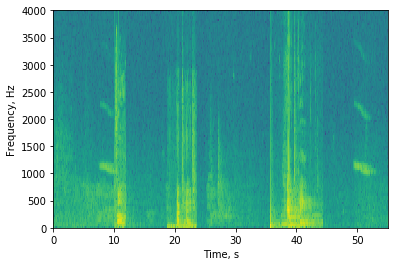
\includegraphics{output_19_0}
    \end{center}
    { \hspace*{\fill} \\}
    
    \begin{tcolorbox}[breakable, size=fbox, boxrule=1pt, pad at break*=1mm,colback=cellbackground, colframe=cellborder]
\prompt{In}{incolor}{16}{\boxspacing}
\begin{Verbatim}[commandchars=\\\{\}]
\PY{l+s+sd}{\PYZsq{}\PYZsq{}\PYZsq{}}
\PY{l+s+sd}{Spectrum: }
\PY{l+s+sd}{columns: periodograms of successive segments (timesteps after the transform)}
\PY{l+s+sd}{rows: frequencies}
\PY{l+s+sd}{\PYZsq{}\PYZsq{}\PYZsq{}} 
\PY{c+c1}{\PYZsh{} Retrieve number of frequencies in the input}
\PY{n}{n\PYZus{}freq} \PY{o}{=} \PY{n}{spectrum}\PY{o}{.}\PY{n}{shape}\PY{p}{[}\PY{l+m+mi}{0}\PY{p}{]}
\PY{n+nb}{print}\PY{p}{(}\PY{l+s+s1}{\PYZsq{}}\PY{l+s+s1}{n\PYZus{}freq = }\PY{l+s+s1}{\PYZsq{}}\PY{p}{,} \PY{n}{n\PYZus{}freq}\PY{p}{)}

\PY{c+c1}{\PYZsh{} Retrieve number of timesteps in the input (out of 10 second audio)}
\PY{n}{Tx} \PY{o}{=} \PY{n}{spectrum}\PY{o}{.}\PY{n}{shape}\PY{p}{[}\PY{l+m+mi}{1}\PY{p}{]}
\PY{n+nb}{print}\PY{p}{(}\PY{l+s+s1}{\PYZsq{}}\PY{l+s+s1}{Tx = }\PY{l+s+s1}{\PYZsq{}}\PY{p}{,} \PY{n}{Tx}\PY{p}{)}

\PY{c+c1}{\PYZsh{} Define number of timesteps in the output }
\PY{n}{Ty} \PY{o}{=} \PY{l+m+mi}{1375}
\PY{n+nb}{print}\PY{p}{(}\PY{l+s+s1}{\PYZsq{}}\PY{l+s+s1}{Ty = }\PY{l+s+s1}{\PYZsq{}}\PY{p}{,} \PY{n}{Ty}\PY{p}{)}
\end{Verbatim}
\end{tcolorbox}

    \begin{Verbatim}[commandchars=\\\{\}]
n\_freq =  101
Tx =  5511
Ty =  1375
    \end{Verbatim}

    \hypertarget{training-set-preparation}{%
\subsection{Training set preparation}\label{training-set-preparation}}

    \begin{tcolorbox}[breakable, size=fbox, boxrule=1pt, pad at break*=1mm,colback=cellbackground, colframe=cellborder]
\prompt{In}{incolor}{17}{\boxspacing}
\begin{Verbatim}[commandchars=\\\{\}]
\PY{c+c1}{\PYZsh{} Create a training example }

\PY{k}{def} \PY{n+nf}{create\PYZus{}training\PYZus{}example}\PY{p}{(}\PY{n}{background}\PY{p}{,} \PY{n}{activates}\PY{p}{,} \PY{n}{negatives}\PY{p}{)}\PY{p}{:}
    
    \PY{n}{np}\PY{o}{.}\PY{n}{random}\PY{o}{.}\PY{n}{seed}\PY{p}{(}\PY{l+m+mi}{18}\PY{p}{)}
    
    \PY{c+c1}{\PYZsh{} Make background quieter}
    \PY{n}{background} \PY{o}{=} \PY{n}{background} \PY{o}{\PYZhy{}} \PY{l+m+mi}{20}

    \PY{c+c1}{\PYZsh{} Initialize output vector and list of inserted segments}
    \PY{n}{y} \PY{o}{=} \PY{n}{np}\PY{o}{.}\PY{n}{zeros}\PY{p}{(}\PY{p}{(}\PY{l+m+mi}{1}\PY{p}{,} \PY{n}{Ty}\PY{p}{)}\PY{p}{)}
    \PY{n}{previous\PYZus{}segments} \PY{o}{=} \PY{p}{[}\PY{p}{]}
    
    \PY{c+c1}{\PYZsh{} Select 0\PYZhy{}4 random \PYZdq{}activate\PYZdq{} audio clips from the entire list of \PYZdq{}activates\PYZdq{} recordings}
    \PY{n}{number\PYZus{}of\PYZus{}activates} \PY{o}{=} \PY{n}{np}\PY{o}{.}\PY{n}{random}\PY{o}{.}\PY{n}{randint}\PY{p}{(}\PY{l+m+mi}{0}\PY{p}{,} \PY{l+m+mi}{5}\PY{p}{)}
    \PY{n}{random\PYZus{}indices} \PY{o}{=} \PY{n}{np}\PY{o}{.}\PY{n}{random}\PY{o}{.}\PY{n}{randint}\PY{p}{(}\PY{n+nb}{len}\PY{p}{(}\PY{n}{activates}\PY{p}{)}\PY{p}{,} \PY{n}{size}\PY{o}{=}\PY{n}{number\PYZus{}of\PYZus{}activates}\PY{p}{)}
    \PY{n}{random\PYZus{}activates} \PY{o}{=} \PY{p}{[}\PY{n}{activates}\PY{p}{[}\PY{n}{i}\PY{p}{]} \PY{k}{for} \PY{n}{i} \PY{o+ow}{in} \PY{n}{random\PYZus{}indices}\PY{p}{]}
    
    \PY{c+c1}{\PYZsh{} Iterate over randomly selected activate clips}
    \PY{k}{for} \PY{n}{random\PYZus{}activate} \PY{o+ow}{in} \PY{n}{random\PYZus{}activates}\PY{p}{:}
       
        \PY{c+c1}{\PYZsh{} Insert \PYZdq{}activate\PYZdq{} clips to background clip}
        \PY{n}{background}\PY{p}{,} \PY{n}{segment\PYZus{}time} \PY{o}{=} \PY{n}{insert\PYZus{}audio\PYZus{}clip}\PY{p}{(}\PY{n}{background}\PY{p}{,} \PY{n}{random\PYZus{}activate}\PY{p}{,} \PY{n}{previous\PYZus{}segments}\PY{p}{)}
        
        \PY{c+c1}{\PYZsh{} Update label vector}
        \PY{n}{y} \PY{o}{=} \PY{n}{insert\PYZus{}ones}\PY{p}{(}\PY{n}{y}\PY{p}{,} \PY{n}{segment\PYZus{}time}\PY{p}{[}\PY{l+m+mi}{1}\PY{p}{]}\PY{p}{)}

    \PY{c+c1}{\PYZsh{} Select 0\PYZhy{}2 random negatives audio recordings from the entire list of \PYZdq{}negatives\PYZdq{} recordings}
    \PY{n}{number\PYZus{}of\PYZus{}negatives} \PY{o}{=} \PY{n}{np}\PY{o}{.}\PY{n}{random}\PY{o}{.}\PY{n}{randint}\PY{p}{(}\PY{l+m+mi}{0}\PY{p}{,} \PY{l+m+mi}{3}\PY{p}{)}
    \PY{n}{random\PYZus{}indices} \PY{o}{=} \PY{n}{np}\PY{o}{.}\PY{n}{random}\PY{o}{.}\PY{n}{randint}\PY{p}{(}\PY{n+nb}{len}\PY{p}{(}\PY{n}{negatives}\PY{p}{)}\PY{p}{,} \PY{n}{size}\PY{o}{=}\PY{n}{number\PYZus{}of\PYZus{}negatives}\PY{p}{)}
    \PY{n}{random\PYZus{}negatives} \PY{o}{=} \PY{p}{[}\PY{n}{negatives}\PY{p}{[}\PY{n}{i}\PY{p}{]} \PY{k}{for} \PY{n}{i} \PY{o+ow}{in} \PY{n}{random\PYZus{}indices}\PY{p}{]}

    \PY{c+c1}{\PYZsh{} Iterate over randomly selected activate clips}
    \PY{k}{for} \PY{n}{random\PYZus{}negative} \PY{o+ow}{in} \PY{n}{random\PYZus{}negatives}\PY{p}{:}
        
        \PY{c+c1}{\PYZsh{} Insert \PYZdq{}negative\PYZdq{} clips to background clip}
        \PY{n}{background}\PY{p}{,} \PY{n}{\PYZus{}} \PY{o}{=} \PY{n}{insert\PYZus{}audio\PYZus{}clip}\PY{p}{(}\PY{n}{background}\PY{p}{,} \PY{n}{random\PYZus{}negative}\PY{p}{,} \PY{n}{previous\PYZus{}segments}\PY{p}{)}
    
    \PY{c+c1}{\PYZsh{} Standardize the volume of the audio clip }
    \PY{n}{target\PYZus{}dBFS} \PY{o}{=} \PY{o}{\PYZhy{}}\PY{l+m+mf}{20.0}
    \PY{n}{change\PYZus{}in\PYZus{}dBFS} \PY{o}{=} \PY{n}{target\PYZus{}dBFS} \PY{o}{\PYZhy{}} \PY{n}{background}\PY{o}{.}\PY{n}{dBFS}
    \PY{n}{background}\PY{o}{.}\PY{n}{apply\PYZus{}gain}\PY{p}{(}\PY{n}{change\PYZus{}in\PYZus{}dBFS}\PY{p}{)}
    
    \PY{c+c1}{\PYZsh{} Export new training example }
    \PY{n}{file\PYZus{}handle} \PY{o}{=} \PY{n}{background}\PY{o}{.}\PY{n}{export}\PY{p}{(}\PY{l+s+s2}{\PYZdq{}}\PY{l+s+s2}{new\PYZus{}training\PYZus{}example}\PY{l+s+s2}{\PYZdq{}} \PY{o}{+} \PY{l+s+s2}{\PYZdq{}}\PY{l+s+s2}{.wav}\PY{l+s+s2}{\PYZdq{}}\PY{p}{,} \PY{n+nb}{format}\PY{o}{=}\PY{l+s+s2}{\PYZdq{}}\PY{l+s+s2}{wav}\PY{l+s+s2}{\PYZdq{}}\PY{p}{)}
    
    \PY{c+c1}{\PYZsh{} Get and plot spectrogram of the new recording (background with superposition of positive and negatives)}
    \PY{n}{x} \PY{o}{=} \PY{n}{graph\PYZus{}spectrogram}\PY{p}{(}\PY{l+s+s2}{\PYZdq{}}\PY{l+s+s2}{./new\PYZus{}training\PYZus{}example.wav}\PY{l+s+s2}{\PYZdq{}}\PY{p}{)}
    
    \PY{k}{return} \PY{n}{x}\PY{p}{,} \PY{n}{y}
\end{Verbatim}
\end{tcolorbox}

    \begin{tcolorbox}[breakable, size=fbox, boxrule=1pt, pad at break*=1mm,colback=cellbackground, colframe=cellborder]
\prompt{In}{incolor}{18}{\boxspacing}
\begin{Verbatim}[commandchars=\\\{\}]
\PY{c+c1}{\PYZsh{} Create a training example}
\PY{n}{x}\PY{p}{,} \PY{n}{y} \PY{o}{=} \PY{n}{create\PYZus{}training\PYZus{}example}\PY{p}{(}\PY{n}{backgrounds}\PY{p}{[}\PY{l+m+mi}{1}\PY{p}{]}\PY{p}{,} \PY{n}{activates}\PY{p}{,} \PY{n}{negatives}\PY{p}{)}
\end{Verbatim}
\end{tcolorbox}

    \begin{center}
    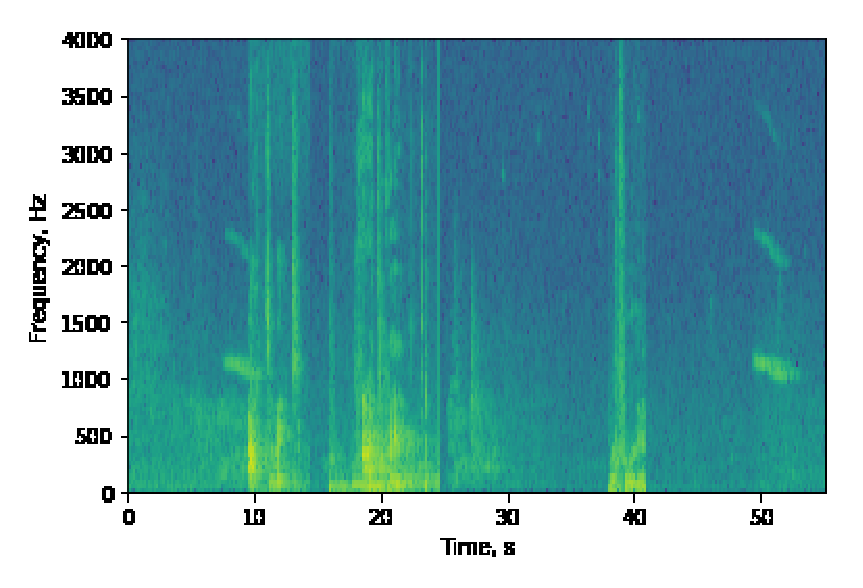
\includegraphics{output_23_0}
    \end{center}
    { \hspace*{\fill} \\}
    
    \begin{tcolorbox}[breakable, size=fbox, boxrule=1pt, pad at break*=1mm,colback=cellbackground, colframe=cellborder]
\prompt{In}{incolor}{19}{\boxspacing}
\begin{Verbatim}[commandchars=\\\{\}]
\PY{c+c1}{\PYZsh{} Load created audio }
\PY{n}{IPython}\PY{o}{.}\PY{n}{display}\PY{o}{.}\PY{n}{Audio}\PY{p}{(}\PY{l+s+s2}{\PYZdq{}}\PY{l+s+s2}{new\PYZus{}training\PYZus{}example.wav}\PY{l+s+s2}{\PYZdq{}}\PY{p}{)}
\end{Verbatim}
\end{tcolorbox}

            \begin{tcolorbox}[breakable, size=fbox, boxrule=.5pt, pad at break*=1mm, opacityfill=0]
\prompt{Out}{outcolor}{19}{\boxspacing}
\begin{Verbatim}[commandchars=\\\{\}]
<IPython.lib.display.Audio object>
\end{Verbatim}
\end{tcolorbox}
        
    \begin{tcolorbox}[breakable, size=fbox, boxrule=1pt, pad at break*=1mm,colback=cellbackground, colframe=cellborder]
\prompt{In}{incolor}{20}{\boxspacing}
\begin{Verbatim}[commandchars=\\\{\}]
\PY{c+c1}{\PYZsh{} Plot the graph showing the }
\PY{n}{plt}\PY{o}{.}\PY{n}{plot}\PY{p}{(}\PY{n}{y}\PY{p}{[}\PY{l+m+mi}{0}\PY{p}{]}\PY{p}{)}

\PY{c+c1}{\PYZsh{} Add axis labels}
\PY{n}{plt}\PY{o}{.}\PY{n}{title}\PY{p}{(}\PY{l+s+s1}{\PYZsq{}}\PY{l+s+s1}{Label for created training example}\PY{l+s+s1}{\PYZsq{}}\PY{p}{)}
\PY{n}{plt}\PY{o}{.}\PY{n}{xlabel}\PY{p}{(}\PY{l+s+s1}{\PYZsq{}}\PY{l+s+s1}{Timesteps}\PY{l+s+s1}{\PYZsq{}}\PY{p}{)}
\PY{n}{plt}\PY{o}{.}\PY{n}{ylabel}\PY{p}{(}\PY{l+s+s1}{\PYZsq{}}\PY{l+s+s1}{Trigger word detected}\PY{l+s+s1}{\PYZsq{}}\PY{p}{)}
\PY{n}{plt}\PY{o}{.}\PY{n}{show}\PY{p}{(}\PY{p}{)}
\end{Verbatim}
\end{tcolorbox}

    \begin{center}
    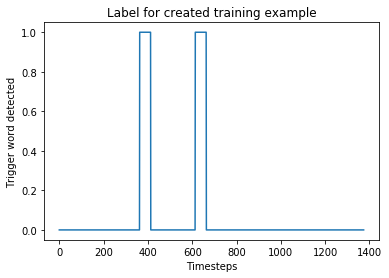
\includegraphics{output_25_0}
    \end{center}
    { \hspace*{\fill} \\}
    
    \begin{tcolorbox}[breakable, size=fbox, boxrule=1pt, pad at break*=1mm,colback=cellbackground, colframe=cellborder]
\prompt{In}{incolor}{21}{\boxspacing}
\begin{Verbatim}[commandchars=\\\{\}]
\PY{c+c1}{\PYZsh{} Create dataset}

\PY{n}{X\PYZus{}train} \PY{o}{=} \PY{n}{np}\PY{o}{.}\PY{n}{zeros}\PY{p}{(}\PY{p}{(}\PY{l+m+mi}{26}\PY{p}{,} \PY{l+m+mi}{5511}\PY{p}{,} \PY{l+m+mi}{101}\PY{p}{)}\PY{p}{)}
\PY{n}{Y\PYZus{}train} \PY{o}{=} \PY{n}{np}\PY{o}{.}\PY{n}{zeros}\PY{p}{(}\PY{p}{(}\PY{l+m+mi}{26}\PY{p}{,} \PY{l+m+mi}{1375}\PY{p}{,} \PY{l+m+mi}{1}\PY{p}{)}\PY{p}{)}

\PY{k}{for} \PY{n}{i} \PY{o+ow}{in} \PY{n+nb}{range}\PY{p}{(}\PY{l+m+mi}{26}\PY{p}{)}\PY{p}{:}
    \PY{n}{background} \PY{o}{=} \PY{n}{backgrounds}\PY{p}{[}\PY{l+m+mi}{0}\PY{p}{]}
    \PY{k}{if} \PY{n}{i} \PY{o}{\PYZgt{}} \PY{l+m+mi}{13}\PY{p}{:}
        \PY{n}{background} \PY{o}{=} \PY{n}{backgrounds}\PY{p}{[}\PY{l+m+mi}{1}\PY{p}{]}
    \PY{n}{x}\PY{p}{,} \PY{n}{y} \PY{o}{=} \PY{n}{create\PYZus{}training\PYZus{}example}\PY{p}{(}\PY{n}{background}\PY{p}{,} \PY{n}{activates}\PY{p}{,} \PY{n}{negatives}\PY{p}{)}
    \PY{n}{X\PYZus{}train}\PY{p}{[}\PY{n}{i}\PY{p}{,} \PY{p}{:}\PY{p}{,} \PY{p}{:}\PY{p}{]} \PY{o}{=} \PY{n}{x}\PY{o}{.}\PY{n}{T}
    \PY{n}{Y\PYZus{}train}\PY{p}{[}\PY{n}{i}\PY{p}{,} \PY{p}{:}\PY{p}{,} \PY{p}{:}\PY{p}{]} \PY{o}{=} \PY{n}{y}\PY{o}{.}\PY{n}{T}
\end{Verbatim}
\end{tcolorbox}

    \begin{Verbatim}[commandchars=\\\{\}]
/Applications/anaconda3/lib/python3.6/site-
packages/matplotlib/axes/\_axes.py:7564: RuntimeWarning: divide by zero
encountered in log10
  Z = 10. * np.log10(spec)
    \end{Verbatim}

    \begin{center}
    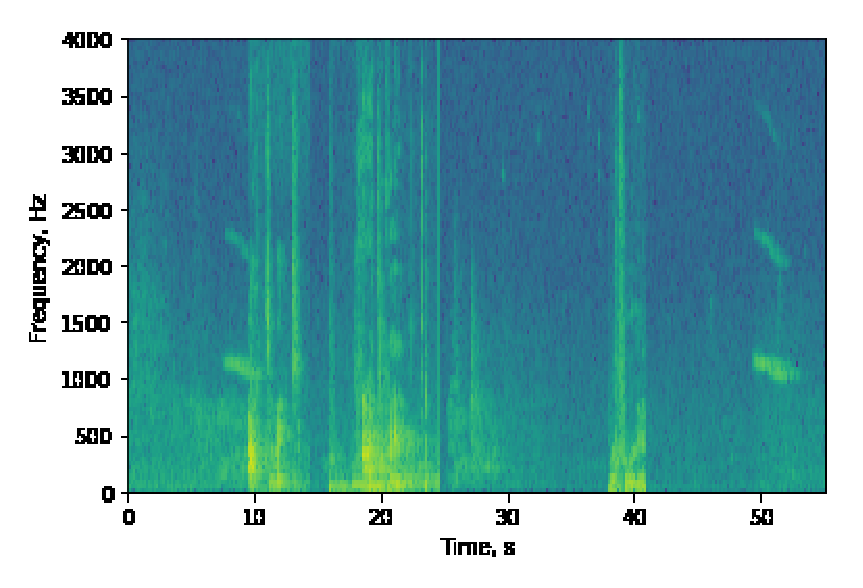
\includegraphics{output_26_1}
    \end{center}
    { \hspace*{\fill} \\}
    
    \begin{tcolorbox}[breakable, size=fbox, boxrule=1pt, pad at break*=1mm,colback=cellbackground, colframe=cellborder]
\prompt{In}{incolor}{22}{\boxspacing}
\begin{Verbatim}[commandchars=\\\{\}]
\PY{n+nb}{print}\PY{p}{(}\PY{l+s+s1}{\PYZsq{}}\PY{l+s+s1}{X\PYZus{}train}\PY{l+s+s1}{\PYZsq{}}\PY{p}{,} \PY{n}{X\PYZus{}train}\PY{o}{.}\PY{n}{shape}\PY{p}{)}
\PY{n+nb}{print}\PY{p}{(}\PY{l+s+s1}{\PYZsq{}}\PY{l+s+s1}{Y\PYZus{}train}\PY{l+s+s1}{\PYZsq{}}\PY{p}{,} \PY{n}{Y\PYZus{}train}\PY{o}{.}\PY{n}{shape}\PY{p}{)}
\end{Verbatim}
\end{tcolorbox}

    \begin{Verbatim}[commandchars=\\\{\}]
X\_train (26, 5511, 101)
Y\_train (26, 1375, 1)
    \end{Verbatim}

    \hypertarget{model-architecture}{%
\subsection{Model architecture}\label{model-architecture}}

    \begin{tcolorbox}[breakable, size=fbox, boxrule=1pt, pad at break*=1mm,colback=cellbackground, colframe=cellborder]
\prompt{In}{incolor}{23}{\boxspacing}
\begin{Verbatim}[commandchars=\\\{\}]
\PY{k+kn}{from} \PY{n+nn}{keras}\PY{n+nn}{.}\PY{n+nn}{models} \PY{k+kn}{import} \PY{n}{Model}\PY{p}{,} \PY{n}{load\PYZus{}model}
\PY{k+kn}{from} \PY{n+nn}{keras}\PY{n+nn}{.}\PY{n+nn}{layers} \PY{k+kn}{import} \PY{n}{Dense}\PY{p}{,} \PY{n}{Activation}\PY{p}{,} \PY{n}{Dropout}\PY{p}{,} \PY{n}{Input}\PY{p}{,} \PY{n}{TimeDistributed}\PY{p}{,} \PY{n}{Conv1D}\PY{p}{,} \PY{n}{GRU}\PY{p}{,} \PY{n}{BatchNormalization}
\PY{k+kn}{from} \PY{n+nn}{keras}\PY{n+nn}{.}\PY{n+nn}{optimizers} \PY{k+kn}{import} \PY{n}{Adam}
\end{Verbatim}
\end{tcolorbox}

    \begin{Verbatim}[commandchars=\\\{\}]
/Applications/anaconda3/lib/python3.6/site-packages/h5py/\_\_init\_\_.py:36:
FutureWarning: Conversion of the second argument of issubdtype from `float` to
`np.floating` is deprecated. In future, it will be treated as `np.float64 ==
np.dtype(float).type`.
  from .\_conv import register\_converters as \_register\_converters
Using TensorFlow backend.
/Applications/anaconda3/lib/python3.6/site-
packages/tensorflow/python/framework/dtypes.py:458: FutureWarning: Passing
(type, 1) or '1type' as a synonym of type is deprecated; in a future version of
numpy, it will be understood as (type, (1,)) / '(1,)type'.
  \_np\_qint8 = np.dtype([("qint8", np.int8, 1)])
/Applications/anaconda3/lib/python3.6/site-
packages/tensorflow/python/framework/dtypes.py:459: FutureWarning: Passing
(type, 1) or '1type' as a synonym of type is deprecated; in a future version of
numpy, it will be understood as (type, (1,)) / '(1,)type'.
  \_np\_quint8 = np.dtype([("quint8", np.uint8, 1)])
/Applications/anaconda3/lib/python3.6/site-
packages/tensorflow/python/framework/dtypes.py:460: FutureWarning: Passing
(type, 1) or '1type' as a synonym of type is deprecated; in a future version of
numpy, it will be understood as (type, (1,)) / '(1,)type'.
  \_np\_qint16 = np.dtype([("qint16", np.int16, 1)])
/Applications/anaconda3/lib/python3.6/site-
packages/tensorflow/python/framework/dtypes.py:461: FutureWarning: Passing
(type, 1) or '1type' as a synonym of type is deprecated; in a future version of
numpy, it will be understood as (type, (1,)) / '(1,)type'.
  \_np\_quint16 = np.dtype([("quint16", np.uint16, 1)])
/Applications/anaconda3/lib/python3.6/site-
packages/tensorflow/python/framework/dtypes.py:462: FutureWarning: Passing
(type, 1) or '1type' as a synonym of type is deprecated; in a future version of
numpy, it will be understood as (type, (1,)) / '(1,)type'.
  \_np\_qint32 = np.dtype([("qint32", np.int32, 1)])
/Applications/anaconda3/lib/python3.6/site-
packages/tensorflow/python/framework/dtypes.py:465: FutureWarning: Passing
(type, 1) or '1type' as a synonym of type is deprecated; in a future version of
numpy, it will be understood as (type, (1,)) / '(1,)type'.
  np\_resource = np.dtype([("resource", np.ubyte, 1)])
    \end{Verbatim}

    \begin{tcolorbox}[breakable, size=fbox, boxrule=1pt, pad at break*=1mm,colback=cellbackground, colframe=cellborder]
\prompt{In}{incolor}{24}{\boxspacing}
\begin{Verbatim}[commandchars=\\\{\}]
\PY{k}{def} \PY{n+nf}{model}\PY{p}{(}\PY{n}{input\PYZus{}shape}\PY{p}{)}\PY{p}{:}
    
    \PY{n}{X\PYZus{}input} \PY{o}{=} \PY{n}{Input}\PY{p}{(}\PY{n}{shape}\PY{o}{=}\PY{n}{input\PYZus{}shape}\PY{p}{)}
    
    \PY{n}{X} \PY{o}{=} \PY{n}{Conv1D}\PY{p}{(}\PY{n}{filters}\PY{o}{=}\PY{l+m+mi}{196}\PY{p}{,} \PY{n}{kernel\PYZus{}size}\PY{o}{=}\PY{l+m+mi}{15}\PY{p}{,} \PY{n}{strides}\PY{o}{=}\PY{l+m+mi}{4}\PY{p}{)}\PY{p}{(}\PY{n}{X\PYZus{}input}\PY{p}{)}
    \PY{n}{X} \PY{o}{=} \PY{n}{BatchNormalization}\PY{p}{(}\PY{p}{)}\PY{p}{(}\PY{n}{X}\PY{p}{)}
    \PY{n}{X} \PY{o}{=} \PY{n}{Activation}\PY{p}{(}\PY{l+s+s1}{\PYZsq{}}\PY{l+s+s1}{relu}\PY{l+s+s1}{\PYZsq{}}\PY{p}{)}\PY{p}{(}\PY{n}{X}\PY{p}{)}
    \PY{n}{X} \PY{o}{=} \PY{n}{Dropout}\PY{p}{(}\PY{l+m+mf}{0.8}\PY{p}{)}\PY{p}{(}\PY{n}{X}\PY{p}{)}
    
    \PY{n}{X}\PY{o}{=} \PY{n}{GRU}\PY{p}{(}\PY{l+m+mi}{128}\PY{p}{,} \PY{n}{return\PYZus{}sequences}\PY{o}{=}\PY{k+kc}{True}\PY{p}{)}\PY{p}{(}\PY{n}{X}\PY{p}{)}
    \PY{n}{X} \PY{o}{=} \PY{n}{Dropout}\PY{p}{(}\PY{l+m+mf}{0.8}\PY{p}{)}\PY{p}{(}\PY{n}{X}\PY{p}{)}
    \PY{n}{X} \PY{o}{=} \PY{n}{BatchNormalization}\PY{p}{(}\PY{p}{)}\PY{p}{(}\PY{n}{X}\PY{p}{)}
    
    \PY{n}{X}\PY{o}{=} \PY{n}{GRU}\PY{p}{(}\PY{l+m+mi}{128}\PY{p}{,} \PY{n}{return\PYZus{}sequences}\PY{o}{=}\PY{k+kc}{True}\PY{p}{)}\PY{p}{(}\PY{n}{X}\PY{p}{)}
    \PY{n}{X} \PY{o}{=} \PY{n}{Dropout}\PY{p}{(}\PY{l+m+mf}{0.8}\PY{p}{)}\PY{p}{(}\PY{n}{X}\PY{p}{)}
    \PY{n}{X} \PY{o}{=} \PY{n}{BatchNormalization}\PY{p}{(}\PY{p}{)}\PY{p}{(}\PY{n}{X}\PY{p}{)}
    \PY{n}{X} \PY{o}{=} \PY{n}{Dropout}\PY{p}{(}\PY{l+m+mf}{0.8}\PY{p}{)}\PY{p}{(}\PY{n}{X}\PY{p}{)}
    
    \PY{n}{X} \PY{o}{=} \PY{n}{TimeDistributed}\PY{p}{(}\PY{n}{Dense}\PY{p}{(}\PY{l+m+mi}{1}\PY{p}{,} \PY{n}{activation}\PY{o}{=}\PY{l+s+s1}{\PYZsq{}}\PY{l+s+s1}{sigmoid}\PY{l+s+s1}{\PYZsq{}}\PY{p}{)}\PY{p}{)}\PY{p}{(}\PY{n}{X}\PY{p}{)}
    
    \PY{n}{model} \PY{o}{=} \PY{n}{Model}\PY{p}{(}\PY{n+nb}{input}\PY{o}{=}\PY{n}{X\PYZus{}input}\PY{p}{,} \PY{n}{outputs}\PY{o}{=}\PY{n}{X}\PY{p}{)}
    
    \PY{k}{return} \PY{n}{model}
\end{Verbatim}
\end{tcolorbox}

    \begin{tcolorbox}[breakable, size=fbox, boxrule=1pt, pad at break*=1mm,colback=cellbackground, colframe=cellborder]
\prompt{In}{incolor}{25}{\boxspacing}
\begin{Verbatim}[commandchars=\\\{\}]
\PY{n}{model} \PY{o}{=} \PY{n}{model}\PY{p}{(}\PY{n}{input\PYZus{}shape}\PY{o}{=}\PY{p}{(}\PY{n}{Tx}\PY{p}{,} \PY{n}{n\PYZus{}freq}\PY{p}{)}\PY{p}{)}
\end{Verbatim}
\end{tcolorbox}

    \begin{Verbatim}[commandchars=\\\{\}]
/Applications/anaconda3/lib/python3.6/site-packages/ipykernel\_launcher.py:21:
UserWarning: Update your `Model` call to the Keras 2 API:
`Model(outputs=Tensor("ti{\ldots}, inputs=Tensor("in{\ldots})`
    \end{Verbatim}

    \begin{tcolorbox}[breakable, size=fbox, boxrule=1pt, pad at break*=1mm,colback=cellbackground, colframe=cellborder]
\prompt{In}{incolor}{26}{\boxspacing}
\begin{Verbatim}[commandchars=\\\{\}]
\PY{n}{model}\PY{o}{.}\PY{n}{summary}\PY{p}{(}\PY{p}{)}
\end{Verbatim}
\end{tcolorbox}

    \begin{Verbatim}[commandchars=\\\{\}]
\_\_\_\_\_\_\_\_\_\_\_\_\_\_\_\_\_\_\_\_\_\_\_\_\_\_\_\_\_\_\_\_\_\_\_\_\_\_\_\_\_\_\_\_\_\_\_\_\_\_\_\_\_\_\_\_\_\_\_\_\_\_\_\_\_
Layer (type)                 Output Shape              Param \#
=================================================================
input\_1 (InputLayer)         (None, 5511, 101)         0
\_\_\_\_\_\_\_\_\_\_\_\_\_\_\_\_\_\_\_\_\_\_\_\_\_\_\_\_\_\_\_\_\_\_\_\_\_\_\_\_\_\_\_\_\_\_\_\_\_\_\_\_\_\_\_\_\_\_\_\_\_\_\_\_\_
conv1d\_1 (Conv1D)            (None, 1375, 196)         297136
\_\_\_\_\_\_\_\_\_\_\_\_\_\_\_\_\_\_\_\_\_\_\_\_\_\_\_\_\_\_\_\_\_\_\_\_\_\_\_\_\_\_\_\_\_\_\_\_\_\_\_\_\_\_\_\_\_\_\_\_\_\_\_\_\_
batch\_normalization\_1 (Batch (None, 1375, 196)         784
\_\_\_\_\_\_\_\_\_\_\_\_\_\_\_\_\_\_\_\_\_\_\_\_\_\_\_\_\_\_\_\_\_\_\_\_\_\_\_\_\_\_\_\_\_\_\_\_\_\_\_\_\_\_\_\_\_\_\_\_\_\_\_\_\_
activation\_1 (Activation)    (None, 1375, 196)         0
\_\_\_\_\_\_\_\_\_\_\_\_\_\_\_\_\_\_\_\_\_\_\_\_\_\_\_\_\_\_\_\_\_\_\_\_\_\_\_\_\_\_\_\_\_\_\_\_\_\_\_\_\_\_\_\_\_\_\_\_\_\_\_\_\_
dropout\_1 (Dropout)          (None, 1375, 196)         0
\_\_\_\_\_\_\_\_\_\_\_\_\_\_\_\_\_\_\_\_\_\_\_\_\_\_\_\_\_\_\_\_\_\_\_\_\_\_\_\_\_\_\_\_\_\_\_\_\_\_\_\_\_\_\_\_\_\_\_\_\_\_\_\_\_
gru\_1 (GRU)                  (None, 1375, 128)         124800
\_\_\_\_\_\_\_\_\_\_\_\_\_\_\_\_\_\_\_\_\_\_\_\_\_\_\_\_\_\_\_\_\_\_\_\_\_\_\_\_\_\_\_\_\_\_\_\_\_\_\_\_\_\_\_\_\_\_\_\_\_\_\_\_\_
dropout\_2 (Dropout)          (None, 1375, 128)         0
\_\_\_\_\_\_\_\_\_\_\_\_\_\_\_\_\_\_\_\_\_\_\_\_\_\_\_\_\_\_\_\_\_\_\_\_\_\_\_\_\_\_\_\_\_\_\_\_\_\_\_\_\_\_\_\_\_\_\_\_\_\_\_\_\_
batch\_normalization\_2 (Batch (None, 1375, 128)         512
\_\_\_\_\_\_\_\_\_\_\_\_\_\_\_\_\_\_\_\_\_\_\_\_\_\_\_\_\_\_\_\_\_\_\_\_\_\_\_\_\_\_\_\_\_\_\_\_\_\_\_\_\_\_\_\_\_\_\_\_\_\_\_\_\_
gru\_2 (GRU)                  (None, 1375, 128)         98688
\_\_\_\_\_\_\_\_\_\_\_\_\_\_\_\_\_\_\_\_\_\_\_\_\_\_\_\_\_\_\_\_\_\_\_\_\_\_\_\_\_\_\_\_\_\_\_\_\_\_\_\_\_\_\_\_\_\_\_\_\_\_\_\_\_
dropout\_3 (Dropout)          (None, 1375, 128)         0
\_\_\_\_\_\_\_\_\_\_\_\_\_\_\_\_\_\_\_\_\_\_\_\_\_\_\_\_\_\_\_\_\_\_\_\_\_\_\_\_\_\_\_\_\_\_\_\_\_\_\_\_\_\_\_\_\_\_\_\_\_\_\_\_\_
batch\_normalization\_3 (Batch (None, 1375, 128)         512
\_\_\_\_\_\_\_\_\_\_\_\_\_\_\_\_\_\_\_\_\_\_\_\_\_\_\_\_\_\_\_\_\_\_\_\_\_\_\_\_\_\_\_\_\_\_\_\_\_\_\_\_\_\_\_\_\_\_\_\_\_\_\_\_\_
dropout\_4 (Dropout)          (None, 1375, 128)         0
\_\_\_\_\_\_\_\_\_\_\_\_\_\_\_\_\_\_\_\_\_\_\_\_\_\_\_\_\_\_\_\_\_\_\_\_\_\_\_\_\_\_\_\_\_\_\_\_\_\_\_\_\_\_\_\_\_\_\_\_\_\_\_\_\_
time\_distributed\_1 (TimeDist (None, 1375, 1)           129
=================================================================
Total params: 522,561
Trainable params: 521,657
Non-trainable params: 904
\_\_\_\_\_\_\_\_\_\_\_\_\_\_\_\_\_\_\_\_\_\_\_\_\_\_\_\_\_\_\_\_\_\_\_\_\_\_\_\_\_\_\_\_\_\_\_\_\_\_\_\_\_\_\_\_\_\_\_\_\_\_\_\_\_
    \end{Verbatim}

    \begin{tcolorbox}[breakable, size=fbox, boxrule=1pt, pad at break*=1mm,colback=cellbackground, colframe=cellborder]
\prompt{In}{incolor}{27}{\boxspacing}
\begin{Verbatim}[commandchars=\\\{\}]
\PY{c+c1}{\PYZsh{} Load pretrained model (provided on coursera hub)}
\PY{n}{model} \PY{o}{=} \PY{n}{load\PYZus{}model}\PY{p}{(}\PY{l+s+s1}{\PYZsq{}}\PY{l+s+s1}{./model/tr\PYZus{}model.h5}\PY{l+s+s1}{\PYZsq{}}\PY{p}{)}
\end{Verbatim}
\end{tcolorbox}

    \begin{tcolorbox}[breakable, size=fbox, boxrule=1pt, pad at break*=1mm,colback=cellbackground, colframe=cellborder]
\prompt{In}{incolor}{28}{\boxspacing}
\begin{Verbatim}[commandchars=\\\{\}]
\PY{c+c1}{\PYZsh{} Requirements for the model to load correctly}
\PY{k+kn}{import} \PY{n+nn}{keras} 
\PY{n}{keras}\PY{o}{.}\PY{n}{\PYZus{}\PYZus{}version\PYZus{}\PYZus{}}
\end{Verbatim}
\end{tcolorbox}

            \begin{tcolorbox}[breakable, size=fbox, boxrule=.5pt, pad at break*=1mm, opacityfill=0]
\prompt{Out}{outcolor}{28}{\boxspacing}
\begin{Verbatim}[commandchars=\\\{\}]
'2.0.7'
\end{Verbatim}
\end{tcolorbox}
        
    \begin{tcolorbox}[breakable, size=fbox, boxrule=1pt, pad at break*=1mm,colback=cellbackground, colframe=cellborder]
\prompt{In}{incolor}{29}{\boxspacing}
\begin{Verbatim}[commandchars=\\\{\}]
\PY{k+kn}{import} \PY{n+nn}{tensorflow}
\PY{n}{tensorflow}\PY{o}{.}\PY{n}{\PYZus{}\PYZus{}version\PYZus{}\PYZus{}}
\end{Verbatim}
\end{tcolorbox}

            \begin{tcolorbox}[breakable, size=fbox, boxrule=.5pt, pad at break*=1mm, opacityfill=0]
\prompt{Out}{outcolor}{29}{\boxspacing}
\begin{Verbatim}[commandchars=\\\{\}]
'1.2.1'
\end{Verbatim}
\end{tcolorbox}
        
    \hypertarget{training}{%
\subsection{Training}\label{training}}

    \begin{tcolorbox}[breakable, size=fbox, boxrule=1pt, pad at break*=1mm,colback=cellbackground, colframe=cellborder]
\prompt{In}{incolor}{30}{\boxspacing}
\begin{Verbatim}[commandchars=\\\{\}]
\PY{c+c1}{\PYZsh{} Define optimizer }
\PY{n}{optimizer} \PY{o}{=} \PY{n}{Adam}\PY{p}{(}\PY{n}{lr}\PY{o}{=}\PY{l+m+mf}{0.0001}\PY{p}{,} \PY{n}{beta\PYZus{}1}\PY{o}{=}\PY{l+m+mf}{0.9}\PY{p}{,} \PY{n}{beta\PYZus{}2}\PY{o}{=}\PY{l+m+mf}{0.999}\PY{p}{,} \PY{n}{decay}\PY{o}{=}\PY{l+m+mf}{0.01}\PY{p}{)}
\end{Verbatim}
\end{tcolorbox}

    \begin{tcolorbox}[breakable, size=fbox, boxrule=1pt, pad at break*=1mm,colback=cellbackground, colframe=cellborder]
\prompt{In}{incolor}{31}{\boxspacing}
\begin{Verbatim}[commandchars=\\\{\}]
\PY{c+c1}{\PYZsh{} Compile the model }
\PY{n}{model}\PY{o}{.}\PY{n}{compile}\PY{p}{(}\PY{n}{loss}\PY{o}{=}\PY{l+s+s1}{\PYZsq{}}\PY{l+s+s1}{binary\PYZus{}crossentropy}\PY{l+s+s1}{\PYZsq{}}\PY{p}{,} \PY{n}{optimizer}\PY{o}{=}\PY{n}{optimizer}\PY{p}{,} \PY{n}{metrics}\PY{o}{=}\PY{p}{[}\PY{l+s+s1}{\PYZsq{}}\PY{l+s+s1}{accuracy}\PY{l+s+s1}{\PYZsq{}}\PY{p}{]}\PY{p}{)}
\end{Verbatim}
\end{tcolorbox}

    \begin{tcolorbox}[breakable, size=fbox, boxrule=1pt, pad at break*=1mm,colback=cellbackground, colframe=cellborder]
\prompt{In}{incolor}{32}{\boxspacing}
\begin{Verbatim}[commandchars=\\\{\}]
\PY{c+c1}{\PYZsh{} Train the model }
\PY{n}{model}\PY{o}{.}\PY{n}{fit}\PY{p}{(}\PY{n}{X\PYZus{}train}\PY{p}{,} \PY{n}{Y\PYZus{}train}\PY{p}{,} \PY{n}{batch\PYZus{}size}\PY{o}{=}\PY{l+m+mi}{5}\PY{p}{,} \PY{n}{epochs}\PY{o}{=}\PY{l+m+mi}{1}\PY{p}{)}
\end{Verbatim}
\end{tcolorbox}

    \begin{Verbatim}[commandchars=\\\{\}]
Epoch 1/1
26/26 [==============================] - 14s - loss: 0.2951 - acc: 0.9144
    \end{Verbatim}

            \begin{tcolorbox}[breakable, size=fbox, boxrule=.5pt, pad at break*=1mm, opacityfill=0]
\prompt{Out}{outcolor}{32}{\boxspacing}
\begin{Verbatim}[commandchars=\\\{\}]
<keras.callbacks.History at 0xd32abbda0>
\end{Verbatim}
\end{tcolorbox}
        
    \hypertarget{validation}{%
\subsection{Validation}\label{validation}}

    \begin{tcolorbox}[breakable, size=fbox, boxrule=1pt, pad at break*=1mm,colback=cellbackground, colframe=cellborder]
\prompt{In}{incolor}{33}{\boxspacing}
\begin{Verbatim}[commandchars=\\\{\}]
\PY{c+c1}{\PYZsh{}\PYZsh{} Load dev set (found here: https://gitlab\PYZhy{}cw9.centralesupelec.fr/codingweeksstaff/cs\PYZus{}codingweek\PYZus{}audio/tree/master/trigger\PYZus{}word\PYZus{}detection/XY\PYZus{}val)}
\PY{n}{X\PYZus{}dev} \PY{o}{=} \PY{n}{np}\PY{o}{.}\PY{n}{load}\PY{p}{(}\PY{l+s+s1}{\PYZsq{}}\PY{l+s+s1}{./dev/X\PYZus{}dev.npy}\PY{l+s+s1}{\PYZsq{}}\PY{p}{)}
\PY{n}{Y\PYZus{}dev} \PY{o}{=} \PY{n}{np}\PY{o}{.}\PY{n}{load}\PY{p}{(}\PY{l+s+s1}{\PYZsq{}}\PY{l+s+s1}{./dev/Y\PYZus{}dev.npy}\PY{l+s+s1}{\PYZsq{}}\PY{p}{)}
\end{Verbatim}
\end{tcolorbox}

    \begin{tcolorbox}[breakable, size=fbox, boxrule=1pt, pad at break*=1mm,colback=cellbackground, colframe=cellborder]
\prompt{In}{incolor}{34}{\boxspacing}
\begin{Verbatim}[commandchars=\\\{\}]
\PY{c+c1}{\PYZsh{} Evaluate model on dev set }
\PY{n}{loss}\PY{p}{,} \PY{n}{acc} \PY{o}{=} \PY{n}{model}\PY{o}{.}\PY{n}{evaluate}\PY{p}{(}\PY{n}{X\PYZus{}dev}\PY{p}{,} \PY{n}{Y\PYZus{}dev}\PY{p}{)}
\PY{n+nb}{print}\PY{p}{(}\PY{n}{acc}\PY{p}{)}
\end{Verbatim}
\end{tcolorbox}

    \begin{Verbatim}[commandchars=\\\{\}]
25/25 [==============================] - 2s
0.9499345421791077
    \end{Verbatim}

    \hypertarget{testing}{%
\subsection{Testing}\label{testing}}

    \begin{tcolorbox}[breakable, size=fbox, boxrule=1pt, pad at break*=1mm,colback=cellbackground, colframe=cellborder]
\prompt{In}{incolor}{35}{\boxspacing}
\begin{Verbatim}[commandchars=\\\{\}]
\PY{c+c1}{\PYZsh{} Helper function: make predictions }

\PY{k}{def} \PY{n+nf}{detect\PYZus{}triggerword}\PY{p}{(}\PY{n}{filename}\PY{p}{)}\PY{p}{:}
    
    \PY{c+c1}{\PYZsh{} Plot spectrogram on the first subplot}
    \PY{n}{plt}\PY{o}{.}\PY{n}{subplot}\PY{p}{(}\PY{l+m+mi}{2}\PY{p}{,}\PY{l+m+mi}{1}\PY{p}{,}\PY{l+m+mi}{1}\PY{p}{)}
    
    \PY{c+c1}{\PYZsh{} Compute spectrum of the file}
    \PY{n}{x} \PY{o}{=} \PY{n}{graph\PYZus{}spectrogram}\PY{p}{(}\PY{n}{filename}\PY{p}{)}
    
    \PY{c+c1}{\PYZsh{} Convert spectrum format to coincide with model input format}
    \PY{n}{x} \PY{o}{=} \PY{n}{x}\PY{o}{.}\PY{n}{T}
    \PY{n}{x} \PY{o}{=} \PY{n}{np}\PY{o}{.}\PY{n}{expand\PYZus{}dims}\PY{p}{(}\PY{n}{x}\PY{p}{,} \PY{n}{axis}\PY{o}{=}\PY{l+m+mi}{0}\PY{p}{)}
    
    \PY{c+c1}{\PYZsh{} Make predictions}
    \PY{n}{predictions} \PY{o}{=} \PY{n}{model}\PY{o}{.}\PY{n}{predict}\PY{p}{(}\PY{n}{x}\PY{p}{)}
    
    \PY{c+c1}{\PYZsh{} Plot predictions on the second subplot}
    \PY{n}{ax2} \PY{o}{=} \PY{n}{plt}\PY{o}{.}\PY{n}{subplot}\PY{p}{(}\PY{l+m+mi}{2}\PY{p}{,}\PY{l+m+mi}{1}\PY{p}{,}\PY{l+m+mi}{2}\PY{p}{)}
    \PY{n}{ax2}\PY{o}{.}\PY{n}{plot}\PY{p}{(}\PY{n}{predictions}\PY{p}{[}\PY{l+m+mi}{0}\PY{p}{,} \PY{p}{:}\PY{p}{,} \PY{l+m+mi}{0}\PY{p}{]}\PY{p}{)}
    \PY{n}{plt}\PY{o}{.}\PY{n}{ylabel}\PY{p}{(}\PY{l+s+s1}{\PYZsq{}}\PY{l+s+s1}{probability}\PY{l+s+s1}{\PYZsq{}}\PY{p}{)}
    \PY{n}{plt}\PY{o}{.}\PY{n}{ylim}\PY{p}{(}\PY{l+m+mi}{0}\PY{p}{,} \PY{l+m+mi}{1}\PY{p}{)} 
    \PY{n}{plt}\PY{o}{.}\PY{n}{show}\PY{p}{(}\PY{p}{)}
    
    \PY{k}{return} \PY{n}{predictions}
\end{Verbatim}
\end{tcolorbox}

    \begin{tcolorbox}[breakable, size=fbox, boxrule=1pt, pad at break*=1mm,colback=cellbackground, colframe=cellborder]
\prompt{In}{incolor}{36}{\boxspacing}
\begin{Verbatim}[commandchars=\\\{\}]
\PY{c+c1}{\PYZsh{} Helper function: add the sound of a chime when the trigger word is detected }

\PY{n}{chime\PYZus{}file} \PY{o}{=} \PY{l+s+s1}{\PYZsq{}}\PY{l+s+s1}{./audio\PYZus{}examples/chime.wav}\PY{l+s+s1}{\PYZsq{}}

\PY{k}{def} \PY{n+nf}{chime\PYZus{}on\PYZus{}activate}\PY{p}{(}\PY{n}{filename}\PY{p}{,} \PY{n}{predictions}\PY{p}{,} \PY{n}{threshold}\PY{p}{)}\PY{p}{:}
    
    \PY{c+c1}{\PYZsh{} Open the audio file and chime file}
    \PY{n}{audio\PYZus{}clip} \PY{o}{=} \PY{n}{AudioSegment}\PY{o}{.}\PY{n}{from\PYZus{}wav}\PY{p}{(}\PY{n}{filename}\PY{p}{)}
    
    \PY{n}{chime} \PY{o}{=} \PY{n}{AudioSegment}\PY{o}{.}\PY{n}{from\PYZus{}wav}\PY{p}{(}\PY{n}{chime\PYZus{}file}\PY{p}{)}
    
    \PY{c+c1}{\PYZsh{} Retrieve amount of timesteps}
    \PY{n}{Ty} \PY{o}{=} \PY{n}{predictions}\PY{o}{.}\PY{n}{shape}\PY{p}{[}\PY{l+m+mi}{1}\PY{p}{]}
   
    \PY{c+c1}{\PYZsh{} Initialize }
    \PY{n}{consecutive\PYZus{}timesteps} \PY{o}{=} \PY{l+m+mi}{0}
    
    \PY{k}{for} \PY{n}{i} \PY{o+ow}{in} \PY{n+nb}{range}\PY{p}{(}\PY{n}{Ty}\PY{p}{)}\PY{p}{:}

        \PY{n}{consecutive\PYZus{}timesteps} \PY{o}{+}\PY{o}{=} \PY{l+m+mi}{1}
        
        \PY{c+c1}{\PYZsh{} Add sound of a chime, prediction prob is higher than the threshold}
        \PY{k}{if} \PY{n}{predictions}\PY{p}{[}\PY{l+m+mi}{0}\PY{p}{,} \PY{n}{i}\PY{p}{,} \PY{l+m+mi}{0}\PY{p}{]} \PY{o}{\PYZgt{}} \PY{n}{threshold}\PY{p}{:}
            \PY{k}{if} \PY{n}{consecutive\PYZus{}timesteps} \PY{o}{\PYZgt{}} \PY{l+m+mi}{150}\PY{p}{:}
                
                \PY{c+c1}{\PYZsh{} Avoid adding multiple chimes for the same trigger word}
                \PY{n}{audio\PYZus{}clip} \PY{o}{=} \PY{n}{audio\PYZus{}clip}\PY{o}{.}\PY{n}{overlay}\PY{p}{(}\PY{n}{chime}\PY{p}{,} \PY{n}{position}\PY{o}{=}\PY{p}{(}\PY{p}{(}\PY{n}{i} \PY{o}{/} \PY{n}{Ty}\PY{p}{)} \PY{o}{*} \PY{n}{audio\PYZus{}clip}\PY{o}{.}\PY{n}{duration\PYZus{}seconds}\PY{p}{)}\PY{o}{*}\PY{l+m+mi}{1000}\PY{p}{)}
                
                \PY{n}{consecutive\PYZus{}timesteps} \PY{o}{=} \PY{l+m+mi}{0}
    
    \PY{c+c1}{\PYZsh{} Export modified audio}
    \PY{n}{path}\PY{p}{,} \PY{n}{file\PYZus{}extension} \PY{o}{=} \PY{n}{os}\PY{o}{.}\PY{n}{path}\PY{o}{.}\PY{n}{splitext}\PY{p}{(}\PY{n}{filename}\PY{p}{)}  
    \PY{n}{audio\PYZus{}clip}\PY{o}{.}\PY{n}{export}\PY{p}{(}\PY{n}{path} \PY{o}{+} \PY{l+s+s1}{\PYZsq{}}\PY{l+s+s1}{\PYZhy{}output.wav}\PY{l+s+s1}{\PYZsq{}}\PY{p}{,} \PY{n+nb}{format}\PY{o}{=}\PY{l+s+s1}{\PYZsq{}}\PY{l+s+s1}{wav}\PY{l+s+s1}{\PYZsq{}}\PY{p}{)}
\end{Verbatim}
\end{tcolorbox}

    \begin{tcolorbox}[breakable, size=fbox, boxrule=1pt, pad at break*=1mm,colback=cellbackground, colframe=cellborder]
\prompt{In}{incolor}{37}{\boxspacing}
\begin{Verbatim}[commandchars=\\\{\}]
\PY{c+c1}{\PYZsh{} Helper function: preprocess the audio to the correct format}

\PY{k}{def} \PY{n+nf}{preprocess\PYZus{}audio}\PY{p}{(}\PY{n}{filename}\PY{p}{)}\PY{p}{:}
    
    \PY{c+c1}{\PYZsh{} Trim or pad audio segment to 10000ms}
    \PY{n}{padding} \PY{o}{=} \PY{n}{AudioSegment}\PY{o}{.}\PY{n}{silent}\PY{p}{(}\PY{n}{duration}\PY{o}{=}\PY{l+m+mi}{10000}\PY{p}{)}
    \PY{n}{segment} \PY{o}{=} \PY{n}{AudioSegment}\PY{o}{.}\PY{n}{from\PYZus{}wav}\PY{p}{(}\PY{n}{filename}\PY{p}{)}\PY{p}{[}\PY{p}{:}\PY{l+m+mi}{10000}\PY{p}{]}
    \PY{n}{segment} \PY{o}{=} \PY{n}{padding}\PY{o}{.}\PY{n}{overlay}\PY{p}{(}\PY{n}{segment}\PY{p}{)}
    
    \PY{c+c1}{\PYZsh{} Set frame rate to 44100}
    \PY{n}{segment} \PY{o}{=} \PY{n}{segment}\PY{o}{.}\PY{n}{set\PYZus{}frame\PYZus{}rate}\PY{p}{(}\PY{l+m+mi}{44100}\PY{p}{)}
    
    \PY{c+c1}{\PYZsh{} Export as wav}
    \PY{n}{segment}\PY{o}{.}\PY{n}{export}\PY{p}{(}\PY{n}{filename}\PY{p}{,} \PY{n+nb}{format}\PY{o}{=}\PY{l+s+s1}{\PYZsq{}}\PY{l+s+s1}{wav}\PY{l+s+s1}{\PYZsq{}}\PY{p}{)}
\end{Verbatim}
\end{tcolorbox}

    \begin{tcolorbox}[breakable, size=fbox, boxrule=1pt, pad at break*=1mm,colback=cellbackground, colframe=cellborder]
\prompt{In}{incolor}{38}{\boxspacing}
\begin{Verbatim}[commandchars=\\\{\}]
\PY{c+c1}{\PYZsh{} Perform inference}

\PY{k}{def} \PY{n+nf}{inference}\PY{p}{(}\PY{n}{path}\PY{p}{)}\PY{p}{:}
    
    \PY{n}{prediction} \PY{o}{=} \PY{n}{detect\PYZus{}triggerword}\PY{p}{(}\PY{n}{path}\PY{p}{)}
    \PY{n}{chime\PYZus{}on\PYZus{}activate}\PY{p}{(}\PY{n}{path}\PY{p}{,} \PY{n}{prediction}\PY{p}{,} \PY{l+m+mf}{0.5}\PY{p}{)}
    \PY{n}{path}\PY{p}{,} \PY{n}{file\PYZus{}extention} \PY{o}{=} \PY{n}{os}\PY{o}{.}\PY{n}{path}\PY{o}{.}\PY{n}{splitext}\PY{p}{(}\PY{n}{path}\PY{p}{)}
    \PY{k}{return} \PY{n}{IPython}\PY{o}{.}\PY{n}{display}\PY{o}{.}\PY{n}{Audio}\PY{p}{(}\PY{n}{path} \PY{o}{+} \PY{l+s+s1}{\PYZsq{}}\PY{l+s+s1}{\PYZhy{}output.wav}\PY{l+s+s1}{\PYZsq{}}\PY{p}{)}
\end{Verbatim}
\end{tcolorbox}

    \begin{tcolorbox}[breakable, size=fbox, boxrule=1pt, pad at break*=1mm,colback=cellbackground, colframe=cellborder]
\prompt{In}{incolor}{39}{\boxspacing}
\begin{Verbatim}[commandchars=\\\{\}]
\PY{n}{inference}\PY{p}{(}\PY{l+s+s1}{\PYZsq{}}\PY{l+s+s1}{./test/1.wav}\PY{l+s+s1}{\PYZsq{}}\PY{p}{)} \PY{c+c1}{\PYZsh{} silent audio, no chime}
\end{Verbatim}
\end{tcolorbox}

    \begin{Verbatim}[commandchars=\\\{\}]
/Applications/anaconda3/lib/python3.6/site-
packages/matplotlib/axes/\_axes.py:7564: RuntimeWarning: divide by zero
encountered in log10
  Z = 10. * np.log10(spec)
    \end{Verbatim}

    \begin{center}
    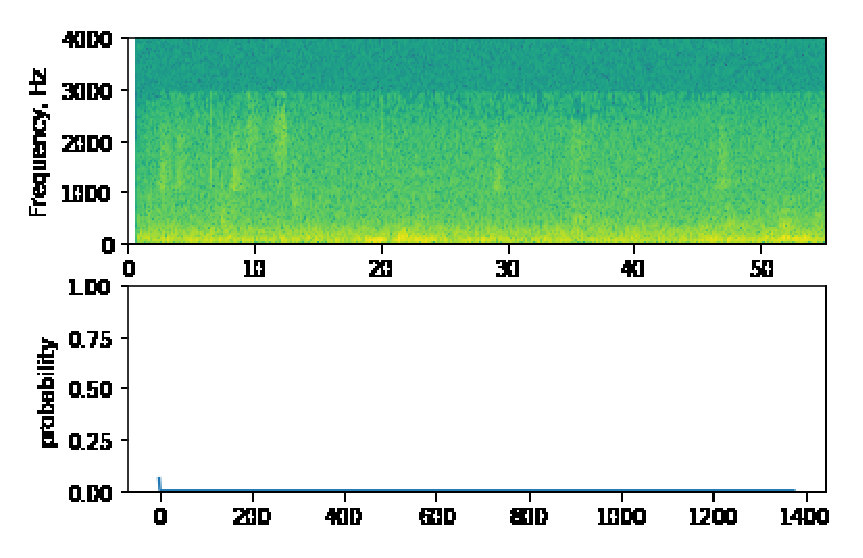
\includegraphics{output_48_1}
    \end{center}
    { \hspace*{\fill} \\}
    
            \begin{tcolorbox}[breakable, size=fbox, boxrule=.5pt, pad at break*=1mm, opacityfill=0]
\prompt{Out}{outcolor}{39}{\boxspacing}
\begin{Verbatim}[commandchars=\\\{\}]
<IPython.lib.display.Audio object>
\end{Verbatim}
\end{tcolorbox}
        
    \begin{tcolorbox}[breakable, size=fbox, boxrule=1pt, pad at break*=1mm,colback=cellbackground, colframe=cellborder]
\prompt{In}{incolor}{40}{\boxspacing}
\begin{Verbatim}[commandchars=\\\{\}]
\PY{n}{inference}\PY{p}{(}\PY{l+s+s1}{\PYZsq{}}\PY{l+s+s1}{./test/2.wav}\PY{l+s+s1}{\PYZsq{}}\PY{p}{)} \PY{c+c1}{\PYZsh{} chimed on \PYZsq{}activate\PYZsq{} and \PYZsq{}algorithm\PYZsq{}}
\end{Verbatim}
\end{tcolorbox}

    \begin{Verbatim}[commandchars=\\\{\}]
/Applications/anaconda3/lib/python3.6/site-
packages/matplotlib/axes/\_axes.py:7564: RuntimeWarning: divide by zero
encountered in log10
  Z = 10. * np.log10(spec)
    \end{Verbatim}

    \begin{center}
    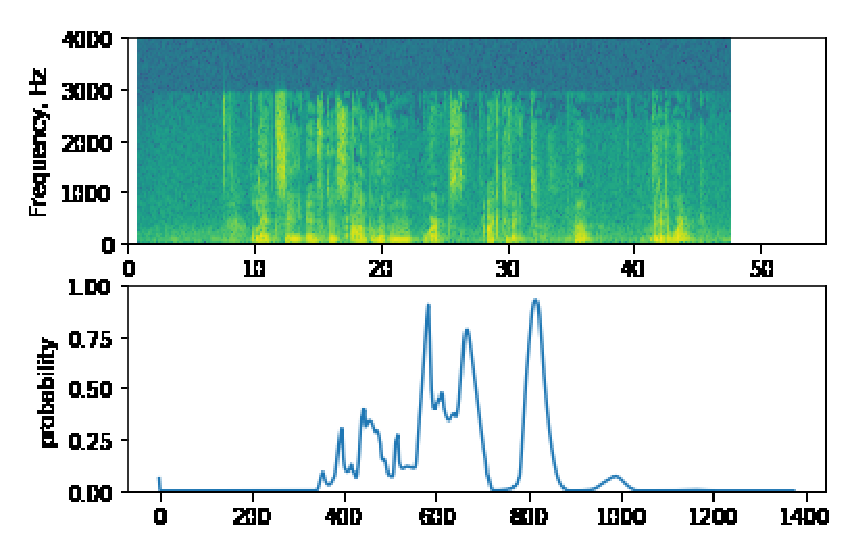
\includegraphics{output_49_1}
    \end{center}
    { \hspace*{\fill} \\}
    
            \begin{tcolorbox}[breakable, size=fbox, boxrule=.5pt, pad at break*=1mm, opacityfill=0]
\prompt{Out}{outcolor}{40}{\boxspacing}
\begin{Verbatim}[commandchars=\\\{\}]
<IPython.lib.display.Audio object>
\end{Verbatim}
\end{tcolorbox}
        
    \begin{tcolorbox}[breakable, size=fbox, boxrule=1pt, pad at break*=1mm,colback=cellbackground, colframe=cellborder]
\prompt{In}{incolor}{41}{\boxspacing}
\begin{Verbatim}[commandchars=\\\{\}]
\PY{n}{inference}\PY{p}{(}\PY{l+s+s1}{\PYZsq{}}\PY{l+s+s1}{./test/3.wav}\PY{l+s+s1}{\PYZsq{}}\PY{p}{)} \PY{c+c1}{\PYZsh{} chimed on \PYZsq{}activate\PYZsq{}}
\end{Verbatim}
\end{tcolorbox}

    \begin{Verbatim}[commandchars=\\\{\}]
/Applications/anaconda3/lib/python3.6/site-
packages/matplotlib/axes/\_axes.py:7564: RuntimeWarning: divide by zero
encountered in log10
  Z = 10. * np.log10(spec)
    \end{Verbatim}

    \begin{center}
    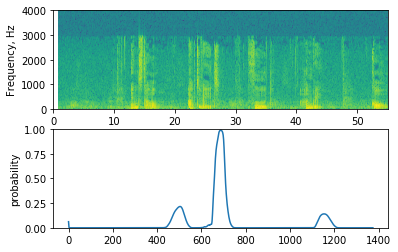
\includegraphics{output_50_1}
    \end{center}
    { \hspace*{\fill} \\}
    
            \begin{tcolorbox}[breakable, size=fbox, boxrule=.5pt, pad at break*=1mm, opacityfill=0]
\prompt{Out}{outcolor}{41}{\boxspacing}
\begin{Verbatim}[commandchars=\\\{\}]
<IPython.lib.display.Audio object>
\end{Verbatim}
\end{tcolorbox}
        
    \begin{tcolorbox}[breakable, size=fbox, boxrule=1pt, pad at break*=1mm,colback=cellbackground, colframe=cellborder]
\prompt{In}{incolor}{42}{\boxspacing}
\begin{Verbatim}[commandchars=\\\{\}]
\PY{n}{inference}\PY{p}{(}\PY{l+s+s1}{\PYZsq{}}\PY{l+s+s1}{./test/4.wav}\PY{l+s+s1}{\PYZsq{}}\PY{p}{)} \PY{c+c1}{\PYZsh{} chimed 3 times on \PYZsq{}activate\PYZsq{}, missed the first one }
\end{Verbatim}
\end{tcolorbox}

    \begin{Verbatim}[commandchars=\\\{\}]
/Applications/anaconda3/lib/python3.6/site-
packages/matplotlib/axes/\_axes.py:7564: RuntimeWarning: divide by zero
encountered in log10
  Z = 10. * np.log10(spec)
    \end{Verbatim}

    \begin{center}
    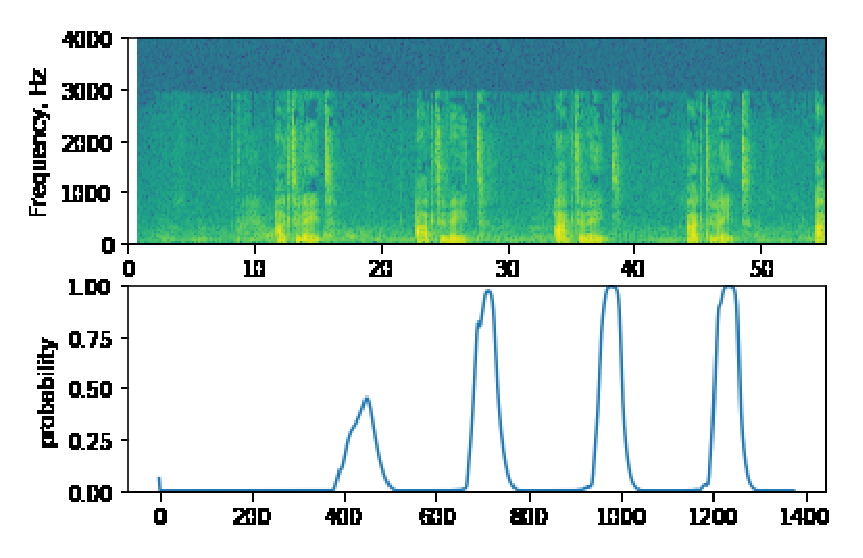
\includegraphics{output_51_1}
    \end{center}
    { \hspace*{\fill} \\}
    
            \begin{tcolorbox}[breakable, size=fbox, boxrule=.5pt, pad at break*=1mm, opacityfill=0]
\prompt{Out}{outcolor}{42}{\boxspacing}
\begin{Verbatim}[commandchars=\\\{\}]
<IPython.lib.display.Audio object>
\end{Verbatim}
\end{tcolorbox}
        
    \begin{tcolorbox}[breakable, size=fbox, boxrule=1pt, pad at break*=1mm,colback=cellbackground, colframe=cellborder]
\prompt{In}{incolor}{43}{\boxspacing}
\begin{Verbatim}[commandchars=\\\{\}]
\PY{n}{inference}\PY{p}{(}\PY{l+s+s1}{\PYZsq{}}\PY{l+s+s1}{./test/5.wav}\PY{l+s+s1}{\PYZsq{}}\PY{p}{)} \PY{c+c1}{\PYZsh{} chimed on \PYZsq{}activate\PYZsq{} and \PYZsq{}iPhone\PYZsq{}}
\end{Verbatim}
\end{tcolorbox}

    \begin{Verbatim}[commandchars=\\\{\}]
/Applications/anaconda3/lib/python3.6/site-
packages/matplotlib/axes/\_axes.py:7564: RuntimeWarning: divide by zero
encountered in log10
  Z = 10. * np.log10(spec)
    \end{Verbatim}

    \begin{center}
    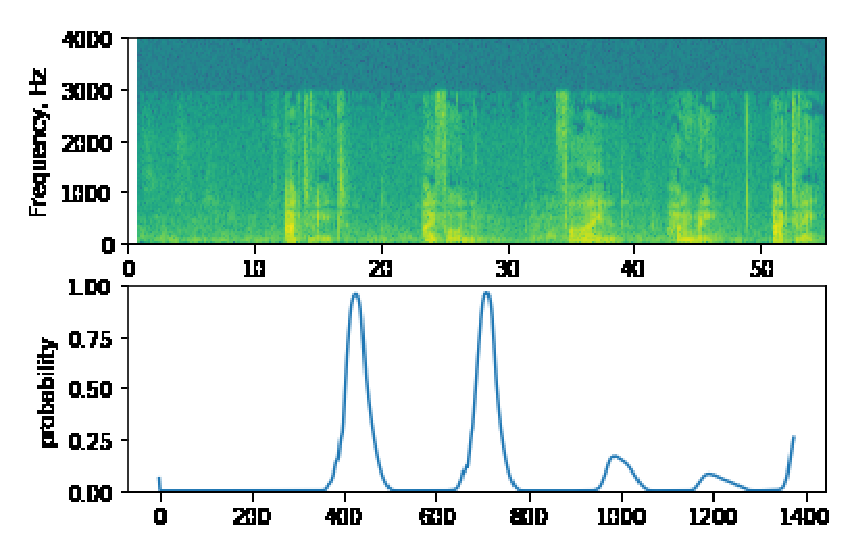
\includegraphics{output_52_1}
    \end{center}
    { \hspace*{\fill} \\}
    
            \begin{tcolorbox}[breakable, size=fbox, boxrule=.5pt, pad at break*=1mm, opacityfill=0]
\prompt{Out}{outcolor}{43}{\boxspacing}
\begin{Verbatim}[commandchars=\\\{\}]
<IPython.lib.display.Audio object>
\end{Verbatim}
\end{tcolorbox}
        
    \begin{tcolorbox}[breakable, size=fbox, boxrule=1pt, pad at break*=1mm,colback=cellbackground, colframe=cellborder]
\prompt{In}{incolor}{44}{\boxspacing}
\begin{Verbatim}[commandchars=\\\{\}]
\PY{n}{inference}\PY{p}{(}\PY{l+s+s1}{\PYZsq{}}\PY{l+s+s1}{./test/6.wav}\PY{l+s+s1}{\PYZsq{}}\PY{p}{)} \PY{c+c1}{\PYZsh{} chimed three times on \PYZsq{}activate\PYZsq{}}
\end{Verbatim}
\end{tcolorbox}

    \begin{Verbatim}[commandchars=\\\{\}]
/Applications/anaconda3/lib/python3.6/site-
packages/matplotlib/axes/\_axes.py:7564: RuntimeWarning: divide by zero
encountered in log10
  Z = 10. * np.log10(spec)
    \end{Verbatim}

    \begin{center}
    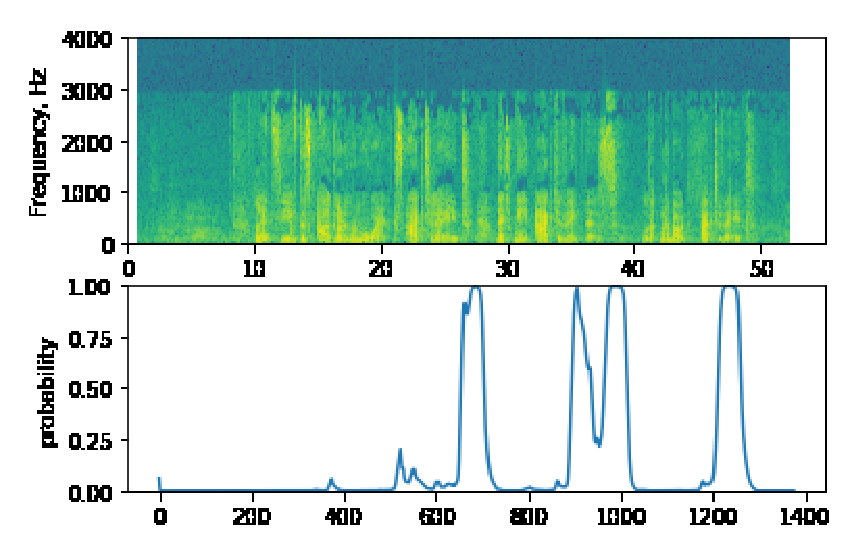
\includegraphics{output_53_1}
    \end{center}
    { \hspace*{\fill} \\}
    
            \begin{tcolorbox}[breakable, size=fbox, boxrule=.5pt, pad at break*=1mm, opacityfill=0]
\prompt{Out}{outcolor}{44}{\boxspacing}
\begin{Verbatim}[commandchars=\\\{\}]
<IPython.lib.display.Audio object>
\end{Verbatim}
\end{tcolorbox}
        
    \begin{tcolorbox}[breakable, size=fbox, boxrule=1pt, pad at break*=1mm,colback=cellbackground, colframe=cellborder]
\prompt{In}{incolor}{45}{\boxspacing}
\begin{Verbatim}[commandchars=\\\{\}]
\PY{n}{inference}\PY{p}{(}\PY{l+s+s1}{\PYZsq{}}\PY{l+s+s1}{./test/7.wav}\PY{l+s+s1}{\PYZsq{}}\PY{p}{)} \PY{c+c1}{\PYZsh{} chimed on \PYZsq{}działa\PYZsq{} and twice on \PYZsq{}activate\PYZsq{}}
\end{Verbatim}
\end{tcolorbox}

    \begin{Verbatim}[commandchars=\\\{\}]
/Applications/anaconda3/lib/python3.6/site-
packages/matplotlib/axes/\_axes.py:7564: RuntimeWarning: divide by zero
encountered in log10
  Z = 10. * np.log10(spec)
    \end{Verbatim}

    \begin{center}
    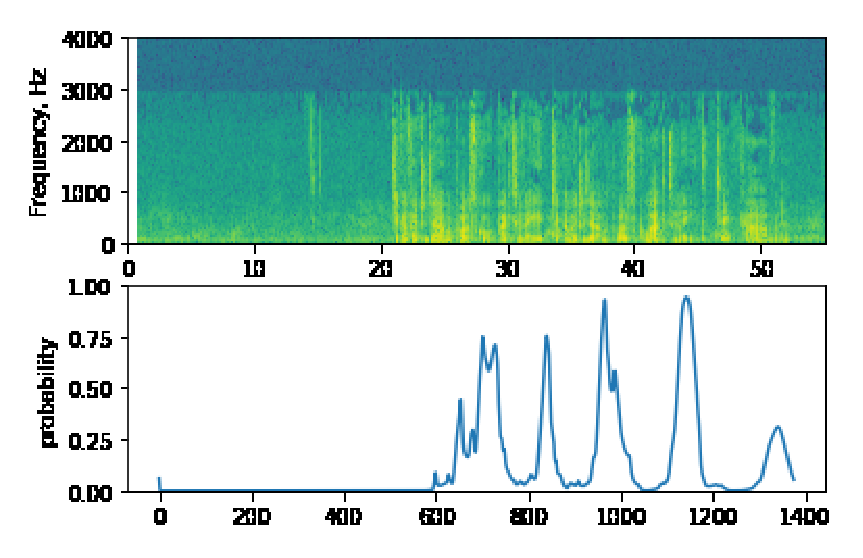
\includegraphics{output_54_1}
    \end{center}
    { \hspace*{\fill} \\}
    
            \begin{tcolorbox}[breakable, size=fbox, boxrule=.5pt, pad at break*=1mm, opacityfill=0]
\prompt{Out}{outcolor}{45}{\boxspacing}
\begin{Verbatim}[commandchars=\\\{\}]
<IPython.lib.display.Audio object>
\end{Verbatim}
\end{tcolorbox}
        
    \begin{tcolorbox}[breakable, size=fbox, boxrule=1pt, pad at break*=1mm,colback=cellbackground, colframe=cellborder]
\prompt{In}{incolor}{46}{\boxspacing}
\begin{Verbatim}[commandchars=\\\{\}]
\PY{n}{inference}\PY{p}{(}\PY{l+s+s1}{\PYZsq{}}\PY{l+s+s1}{./test/8.wav}\PY{l+s+s1}{\PYZsq{}}\PY{p}{)} \PY{c+c1}{\PYZsh{} background noise, chimes twice}
\end{Verbatim}
\end{tcolorbox}

    \begin{Verbatim}[commandchars=\\\{\}]
/Applications/anaconda3/lib/python3.6/site-
packages/matplotlib/axes/\_axes.py:7564: RuntimeWarning: divide by zero
encountered in log10
  Z = 10. * np.log10(spec)
    \end{Verbatim}

    \begin{center}
    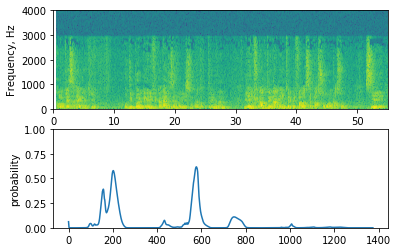
\includegraphics{output_55_1}
    \end{center}
    { \hspace*{\fill} \\}
    
            \begin{tcolorbox}[breakable, size=fbox, boxrule=.5pt, pad at break*=1mm, opacityfill=0]
\prompt{Out}{outcolor}{46}{\boxspacing}
\begin{Verbatim}[commandchars=\\\{\}]
<IPython.lib.display.Audio object>
\end{Verbatim}
\end{tcolorbox}
        
    \begin{tcolorbox}[breakable, size=fbox, boxrule=1pt, pad at break*=1mm,colback=cellbackground, colframe=cellborder]
\prompt{In}{incolor}{ }{\boxspacing}
\begin{Verbatim}[commandchars=\\\{\}]

\end{Verbatim}
\end{tcolorbox}


    % Add a bibliography block to the postdoc
    
    
    
\end{document}
